% Options for packages loaded elsewhere
\PassOptionsToPackage{unicode}{hyperref}
\PassOptionsToPackage{hyphens}{url}
%
\documentclass[
  ignorenonframetext,
]{beamer}
\usepackage{pgfpages}
\setbeamertemplate{caption}[numbered]
\setbeamertemplate{caption label separator}{: }
\setbeamercolor{caption name}{fg=normal text.fg}
\beamertemplatenavigationsymbolsempty
% Prevent slide breaks in the middle of a paragraph
\widowpenalties 1 10000
\raggedbottom
\setbeamertemplate{part page}{
  \centering
  \begin{beamercolorbox}[sep=16pt,center]{part title}
    \usebeamerfont{part title}\insertpart\par
  \end{beamercolorbox}
}
\setbeamertemplate{section page}{
  \centering
  \begin{beamercolorbox}[sep=12pt,center]{part title}
    \usebeamerfont{section title}\insertsection\par
  \end{beamercolorbox}
}
\setbeamertemplate{subsection page}{
  \centering
  \begin{beamercolorbox}[sep=8pt,center]{part title}
    \usebeamerfont{subsection title}\insertsubsection\par
  \end{beamercolorbox}
}
\AtBeginPart{
  \frame{\partpage}
}
\AtBeginSection{
  \ifbibliography
  \else
    \frame{\sectionpage}
  \fi
}
\AtBeginSubsection{
  \frame{\subsectionpage}
}
\usepackage{amsmath,amssymb}
\usepackage{lmodern}
\usepackage{iftex}
\ifPDFTeX
  \usepackage[T1]{fontenc}
  \usepackage[utf8]{inputenc}
  \usepackage{textcomp} % provide euro and other symbols
\else % if luatex or xetex
  \usepackage{unicode-math}
  \defaultfontfeatures{Scale=MatchLowercase}
  \defaultfontfeatures[\rmfamily]{Ligatures=TeX,Scale=1}
\fi
% Use upquote if available, for straight quotes in verbatim environments
\IfFileExists{upquote.sty}{\usepackage{upquote}}{}
\IfFileExists{microtype.sty}{% use microtype if available
  \usepackage[]{microtype}
  \UseMicrotypeSet[protrusion]{basicmath} % disable protrusion for tt fonts
}{}
\makeatletter
\@ifundefined{KOMAClassName}{% if non-KOMA class
  \IfFileExists{parskip.sty}{%
    \usepackage{parskip}
  }{% else
    \setlength{\parindent}{0pt}
    \setlength{\parskip}{6pt plus 2pt minus 1pt}}
}{% if KOMA class
  \KOMAoptions{parskip=half}}
\makeatother
\usepackage{xcolor}
\IfFileExists{xurl.sty}{\usepackage{xurl}}{} % add URL line breaks if available
\IfFileExists{bookmark.sty}{\usepackage{bookmark}}{\usepackage{hyperref}}
\hypersetup{
  hidelinks,
  pdfcreator={LaTeX via pandoc}}
\urlstyle{same} % disable monospaced font for URLs
\newif\ifbibliography
\setlength{\emergencystretch}{3em} % prevent overfull lines
\providecommand{\tightlist}{%
  \setlength{\itemsep}{0pt}\setlength{\parskip}{0pt}}
\setcounter{secnumdepth}{-\maxdimen} % remove section numbering
\newlength{\cslhangindent}
\setlength{\cslhangindent}{1.5em}
\newlength{\csllabelwidth}
\setlength{\csllabelwidth}{3em}
\newlength{\cslentryspacingunit} % times entry-spacing
\setlength{\cslentryspacingunit}{\parskip}
\newenvironment{CSLReferences}[2] % #1 hanging-ident, #2 entry spacing
 {% don't indent paragraphs
  \setlength{\parindent}{0pt}
  % turn on hanging indent if param 1 is 1
  \ifodd #1
  \let\oldpar\par
  \def\par{\hangindent=\cslhangindent\oldpar}
  \fi
  % set entry spacing
  \setlength{\parskip}{#2\cslentryspacingunit}
 }%
 {}
\usepackage{calc}
\newcommand{\CSLBlock}[1]{#1\hfill\break}
\newcommand{\CSLLeftMargin}[1]{\parbox[t]{\csllabelwidth}{#1}}
\newcommand{\CSLRightInline}[1]{\parbox[t]{\linewidth - \csllabelwidth}{#1}\break}
\newcommand{\CSLIndent}[1]{\hspace{\cslhangindent}#1}
\ifLuaTeX
  \usepackage{selnolig}  % disable illegal ligatures
\fi

\author{}
\date{\vspace{-2.5em}}

\begin{document}

\begin{frame}
\begin{block}{Management of herbivorous mites of rose with predatory
mites and Systemic Acquired Resistance}
\protect\hypertarget{management-of-herbivorous-mites-of-rose-with-predatory-mites-and-systemic-acquired-resistance}{}
\begin{itemize}
\tightlist
\item
  \emph{Phyllocoptes fructiphilus} Keifer (Trombidiformes: Eriophyidae)
\item
  Feeds on plants in the genus \emph{Rosa}
\item
  Vector for Rose Rosette Virus (RRV)
\end{itemize}
\end{block}

\begin{block}{RRD Symptoms}
\protect\hypertarget{rrd-symptoms}{}
\begin{figure}
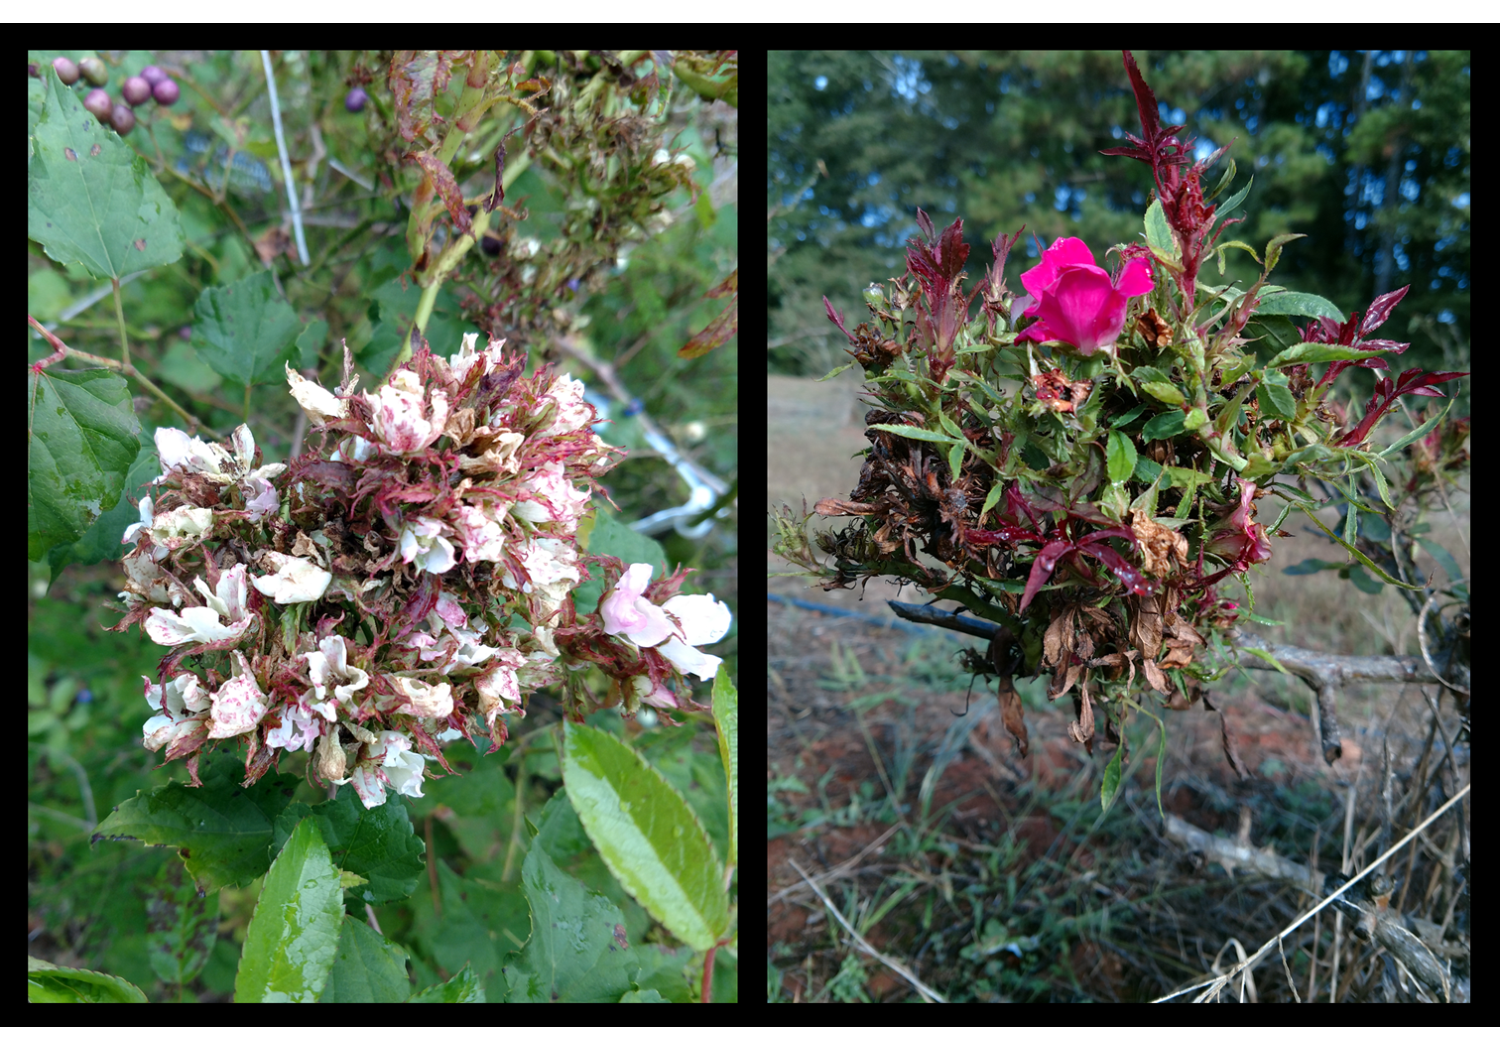
\includegraphics[width=0.8\linewidth]{asa-presentation-2021-denver_files/figure-beamer/rrd-symptoms-1} \caption{Typical symptoms of Rose Rosette Disease (RRD), caused by Rose Rosette Virus: clusters of deformed flowers known as rosettes/witches' brooms, increased thorniness, elongated shoots, reddened leaves and stems. RRD ultimately kills the rose host.}\label{fig:rrd-symptoms}
\end{figure}

\begin{itemize}
\tightlist
\item
  witches' brooms/rosetting, deformed flowers, increased prickle
  density, elongated shoots, reddened leaves and stems, and increased
  die-back which ultimately kills the rose host
  (\protect\hyperlink{ref-Allington1968}{Allington et al. 1968},
  \protect\hyperlink{ref-Tzanetakis2006}{Tzanetakis et al. 2006},
  \protect\hyperlink{ref-Laney2011}{Laney et al. 2011}).
\item
  Most serious disease of roses in the US. RRD and the mite have invaded
  the southeastern US as they followed the range expansion of the
  non-native \emph{Rosa multiflora} (Thunb) towards the coast
  (\protect\hyperlink{ref-Amrine1996}{Amrine Jr 1996},
  \protect\hyperlink{ref-Amrine2002}{2002},
  \protect\hyperlink{ref-Otero-Colina2018}{Otero-Colina et al. 2018}).
\item
  Florida, as the nation's largest producer of roses, has a special
  interest developing methods to better control \emph{P. fructiphilus}
  and RRD. There is a critical need to improve management of \emph{P.
  fructiphilus} and RRD. Unfortunately, few commercially available roses
  have resistance to RRD (\protect\hyperlink{ref-Bello2017}{Di Bello et
  al. 2017}, \protect\hyperlink{ref-Byrne2018}{Byrne et al. 2018}).
\end{itemize}
\end{block}

\begin{block}{\emph{P. fructiphilius} in Florida}
\protect\hypertarget{p.-fructiphilius-in-florida}{}
\begin{figure}[p]
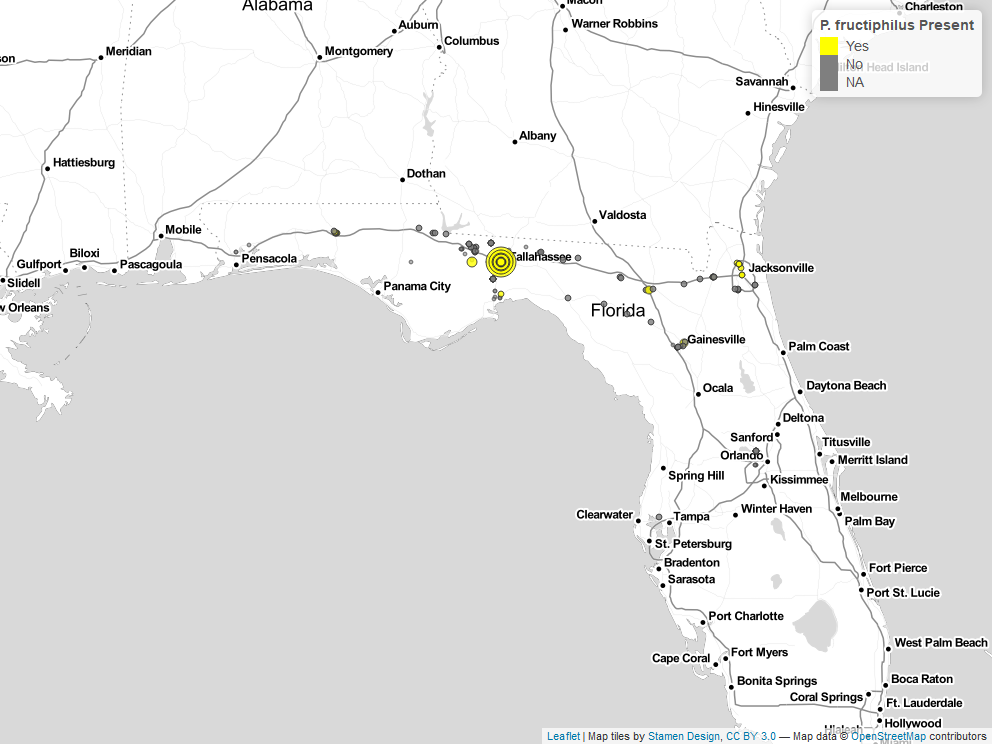
\includegraphics[width=1\linewidth]{figure/rrv_survey_map_fl_pf} \caption{\textit{P. fructiphilus} mites recovered during surveys of roses in Florida, 2017-2021.}\label{fig:survey-map-1}
\end{figure}

\begin{itemize}
\tightlist
\item
  Possibility of introducing RRD from areas where the disease had become
  established, including the neighboring states of Georgia and Alabama
  (\protect\hyperlink{ref-Solo2018}{Solo 2018},
  \protect\hyperlink{ref-Solo2020}{Solo et al. 2020}).
\end{itemize}
\end{block}

\begin{block}{Integrating Pest Management}
\protect\hypertarget{integrating-pest-management}{}
\begin{itemize}
\tightlist
\item
  \emph{P. fructiphilus} is hard to control

  \begin{figure}
  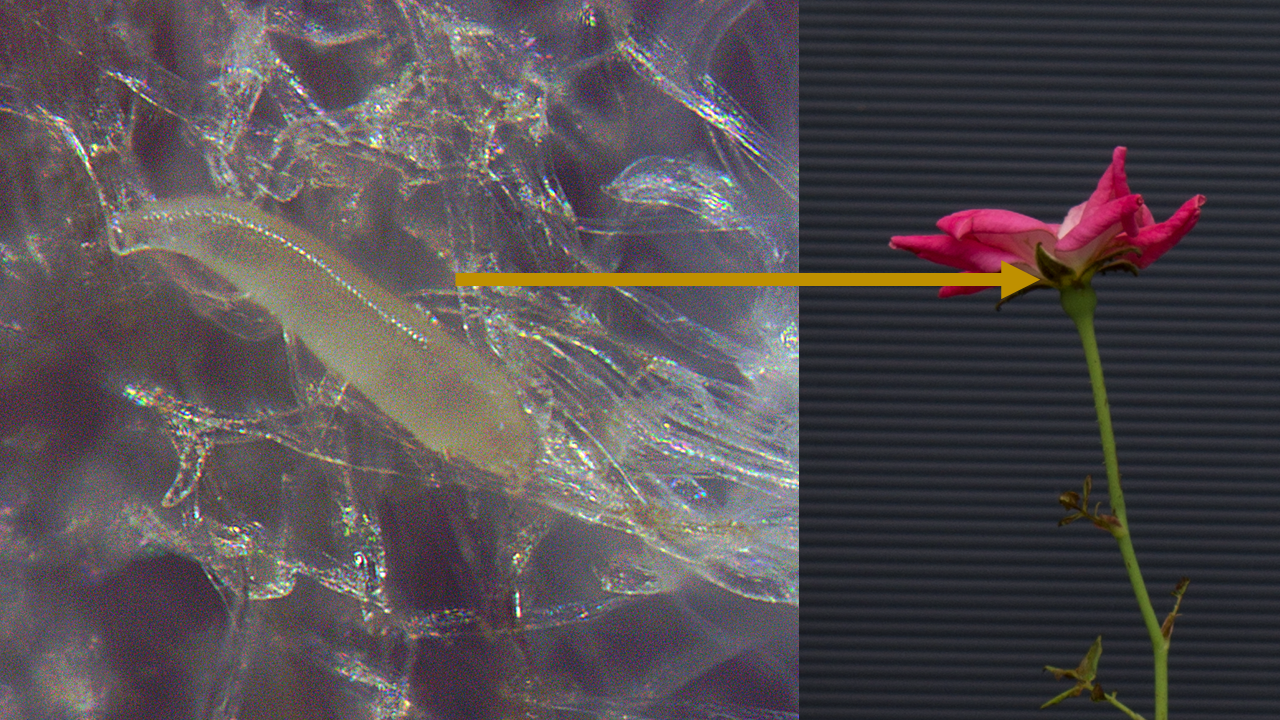
\includegraphics[width=0.8\linewidth]{figure/mite-pfruct-hide} \caption{Illustration of the typical location of \textit{Phyllocoptes fructiphilus} on roses. \textit{P. fructiphilus} are difficult to manage with pesticides due to the protection offered by the sepals.}\label{fig:hiding}
  \end{figure}
\end{itemize}
\end{block}

\begin{block}{Phytoseids an option for control?}
\protect\hypertarget{phytoseids-an-option-for-control}{}
\begin{itemize}
\tightlist
\item
  Small species may be able to find and feed on *P. fructiphilus
\item
  \emph{Amblyseius swirskii} Athias-Henriot (Mesostigmata: Phytoseiidae)
  mites were attracted towards roses which were infected with RRD
\item
  Too large!
\item
  Model organism
\end{itemize}
\end{block}

\begin{block}{What caused the attraction to infected roses?}
\protect\hypertarget{what-caused-the-attraction-to-infected-roses}{}
\begin{itemize}
\tightlist
\item
  Low levels of MeSA from RRV-infected roses
\item
  MeSA attractive to some many predatory mites
\end{itemize}
\end{block}

\begin{block}{MeSA and SAR}
\protect\hypertarget{mesa-and-sar}{}
\begin{itemize}
\tightlist
\item
  MeSA increases when a plant is attacked by herbivores or pathogens,
  derivative of Salicylic Acid
\item
  Systemic Acquired Resistance (SAR), protects distant tissues
\item
  Hypersensitive Response
\item
  Enduring resistance
\item
  Pathogen resistance: fungi, bacteria and viral pathogens
\end{itemize}
\end{block}

\begin{block}{SAR-induction}
\protect\hypertarget{sar-induction}{}
\begin{itemize}
\tightlist
\item
  Induce SAR \emph{before} RRV infection
\item
  acibenzolar-S-methyl (ASM), benzothiadiazole
\item
  ASM used to protect plants from fungal infection
\item
  Chitinase activity in roses (\protect\hyperlink{ref-Suo2001}{Suo and
  Leung 2001})
\item
  Hypersensitive response and SAR interferes with the ability of
  eriophyoid mites to feed or grow on induced plants
  (\protect\hyperlink{ref-Bronner1991a}{Bronner et al. 1991},
  \protect\hyperlink{ref-Westphal1991}{Westphal et al. 1991},
  \protect\hyperlink{ref-Westphal1992}{1992}).
\end{itemize}
\end{block}

\begin{block}{How does SAR-induction affect predators?}
\protect\hypertarget{how-does-sar-induction-affect-predators}{}
\begin{itemize}
\tightlist
\item
  Predatory mites may still be harmed via direct and indirect effects of
  SAR-induction Pappas et al. (\protect\hyperlink{ref-Pappas2017}{2017})
\end{itemize}
\end{block}

\begin{block}{Design: ASM Trials}
\protect\hypertarget{design-asm-trials}{}
\begin{itemize}
\tightlist
\item
  12 weeks, from August to October
\item
  Griffin and Athens, GA
\item
  low and high pest pressure
\item
  Plants inoculated with canes from nearby RRD-infected roses
\item
  Inoculated 1st and 5th weeks of the experiment
\item
  48 Pink Double Knock Out® Roses 1 gallon buckets
\end{itemize}
\end{block}

\begin{block}{Treatments: ASM}
\protect\hypertarget{treatments-asm}{}
\begin{itemize}
\tightlist
\item
  acibenzolar-S-methyl, ASM (Actigard50WG)
\item
  Two rates: 50 \si{\milli\gram}/\si{\liter} (Half rate) and 100
  \si{\milli\gram}/\si{\liter} (High rate)
\item
  Goal: observe the effects of inducing Systemic Acquired Resistance
  (SAR) on \emph{P. fructiphilus}
\item
  Griffin had two controls:
\item
  Kontos (Spirotetramat), label rate (negative control)
\item
  Water (positive control)
\item
  Athens had untreated roses and water as negative controls
\end{itemize}
\end{block}

\begin{block}{Data Collection: ASM}
\protect\hypertarget{data-collection-asm}{}
\begin{itemize}
\tightlist
\item
  Subset of samples weekly
\item
  Each rose plant has been sampled three times.
\item
  Rose/rosebud cuttings \textasciitilde10 cm
\item
  Samples in 50 mL centrifuge tubes
\item
  Washing methods of Monfreda et al.
  (\protect\hyperlink{ref-Monfreda2007}{2007})
\item
  Counted eriophyoid mites
\end{itemize}
\end{block}

\begin{block}{Design: IPM Trials}
\protect\hypertarget{design-ipm-trials}{}
August to October simultaneously in Griffin, GA and Athens, GA. The
Athens site will be given 96 Pink Double Knock Out® Roses (Star Roses
and Plants, West Grove, PA, USA), while Griffin will use 54 roses due to
the smaller plot area available. Bare root roses will be planted 2
months before the trials begin to allow new flush to form. Rose planting
media and environmental conditions will be the same as previously
described.
\end{block}

\begin{block}{Treatments - IPM}
\protect\hypertarget{treatments---ipm}{}
\begin{itemize}
\tightlist
\item
  ASM (Actigard 50WG) and SP2700, (Ninja, SePro)
\item
  \emph{A. swirskii} 2 mini sachets with hooks sachets per rose
\item
  ASM + \emph{A. swirskii}
\item
  Kontos - spirotetramat acaricide as a negative control
\item
  Water - a positive control
\item
  12 weeks, mites applied on the 1st, 5th and 9th week
\item
  Two blocks, 10 plots, 12 roses/plot w/buffer, six roses treated
\end{itemize}
\end{block}

\begin{block}{Plot Design - 2018}
\protect\hypertarget{plot-design---2018}{}
\begin{figure}
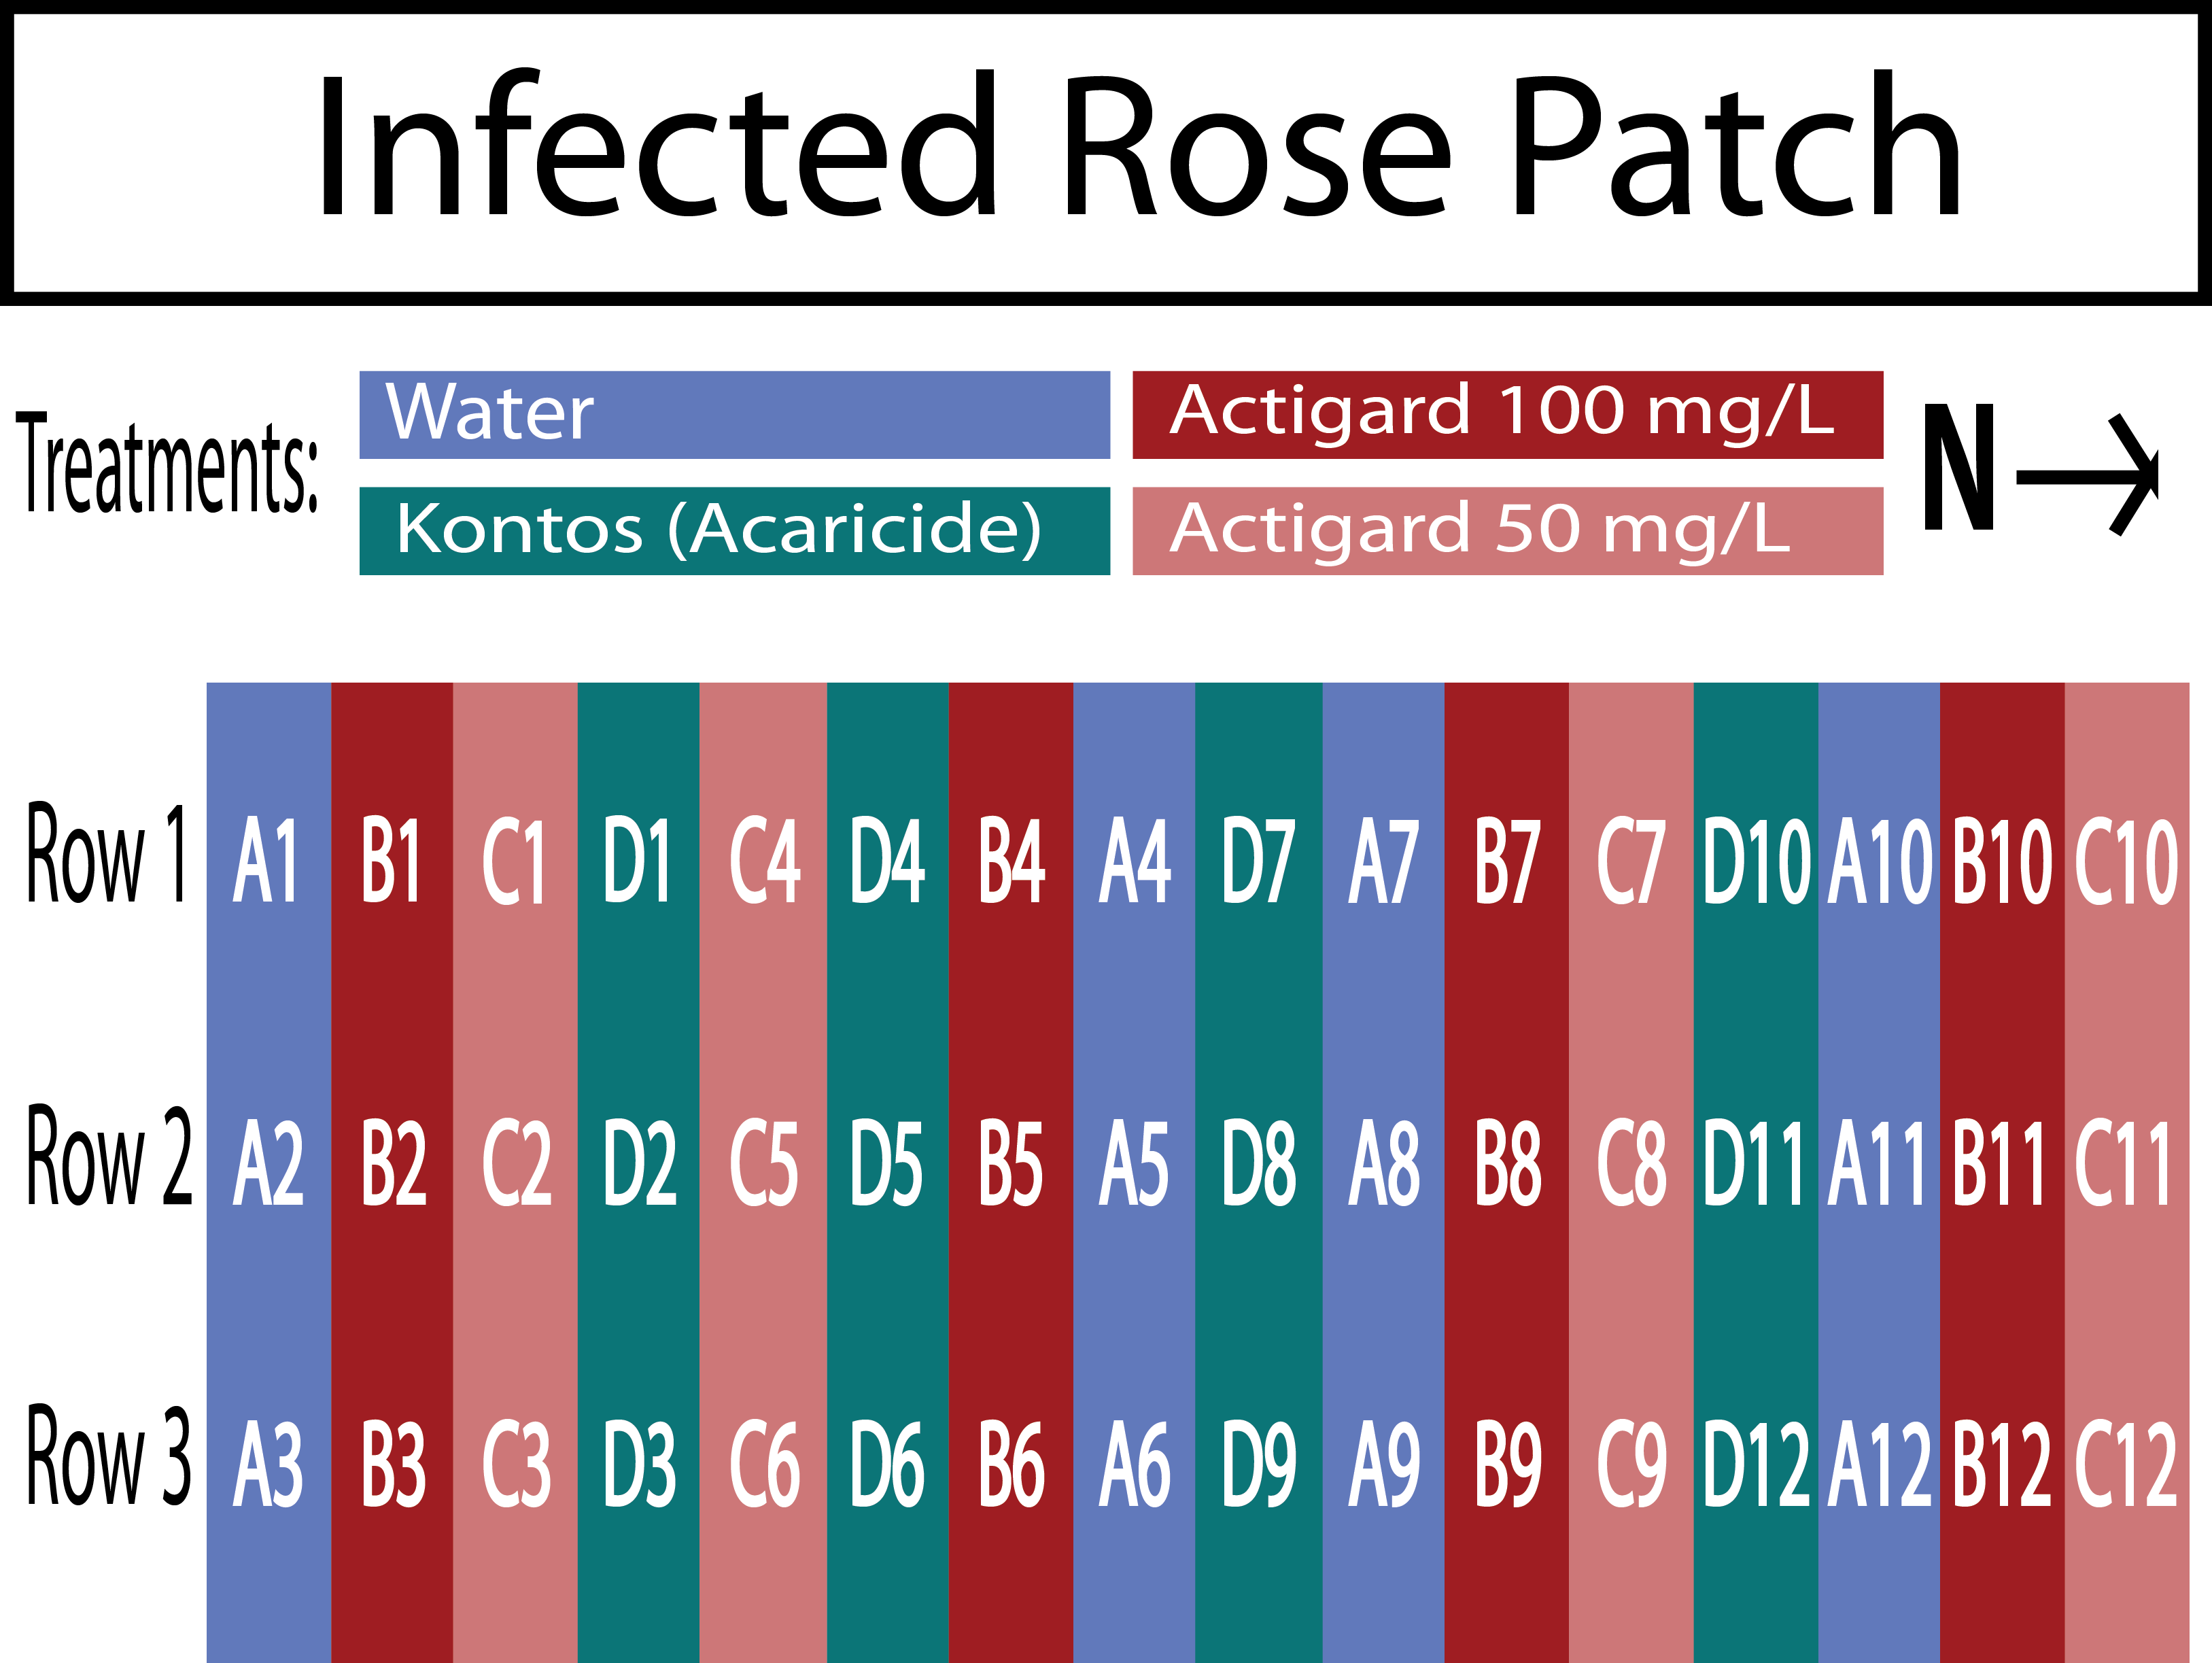
\includegraphics[width=0.8\linewidth]{figure/rrv_asm_plot_2018_griffin} \caption{Field design for testing the potential of Acibenzolar-S-Methyl to reduce populations of \textit{P. fructiphilus} by inducing Systemic Acquired Resistance in Pink Double Knock Out® roses. Trials were conducted for three months from September to December 2019 in Griffin, GA. Four treatments were applied weekly fo 12 weeks: Blue = Water Red = Actigard50WG 100 \si{\milli\gram}/L (High rate),  Pink = Actigard50WG \si{\milli\gram}/L (Half rate) Turquoise = Kontos (Label rate). Flower cuttings were be taken weekly to record \textit{P. fructiphilus} numbers.}\label{fig:unnamed-chunk-1}
\end{figure}
\end{block}

\begin{block}{Plot Design - 2019}
\protect\hypertarget{plot-design---2019}{}
\begin{figure}
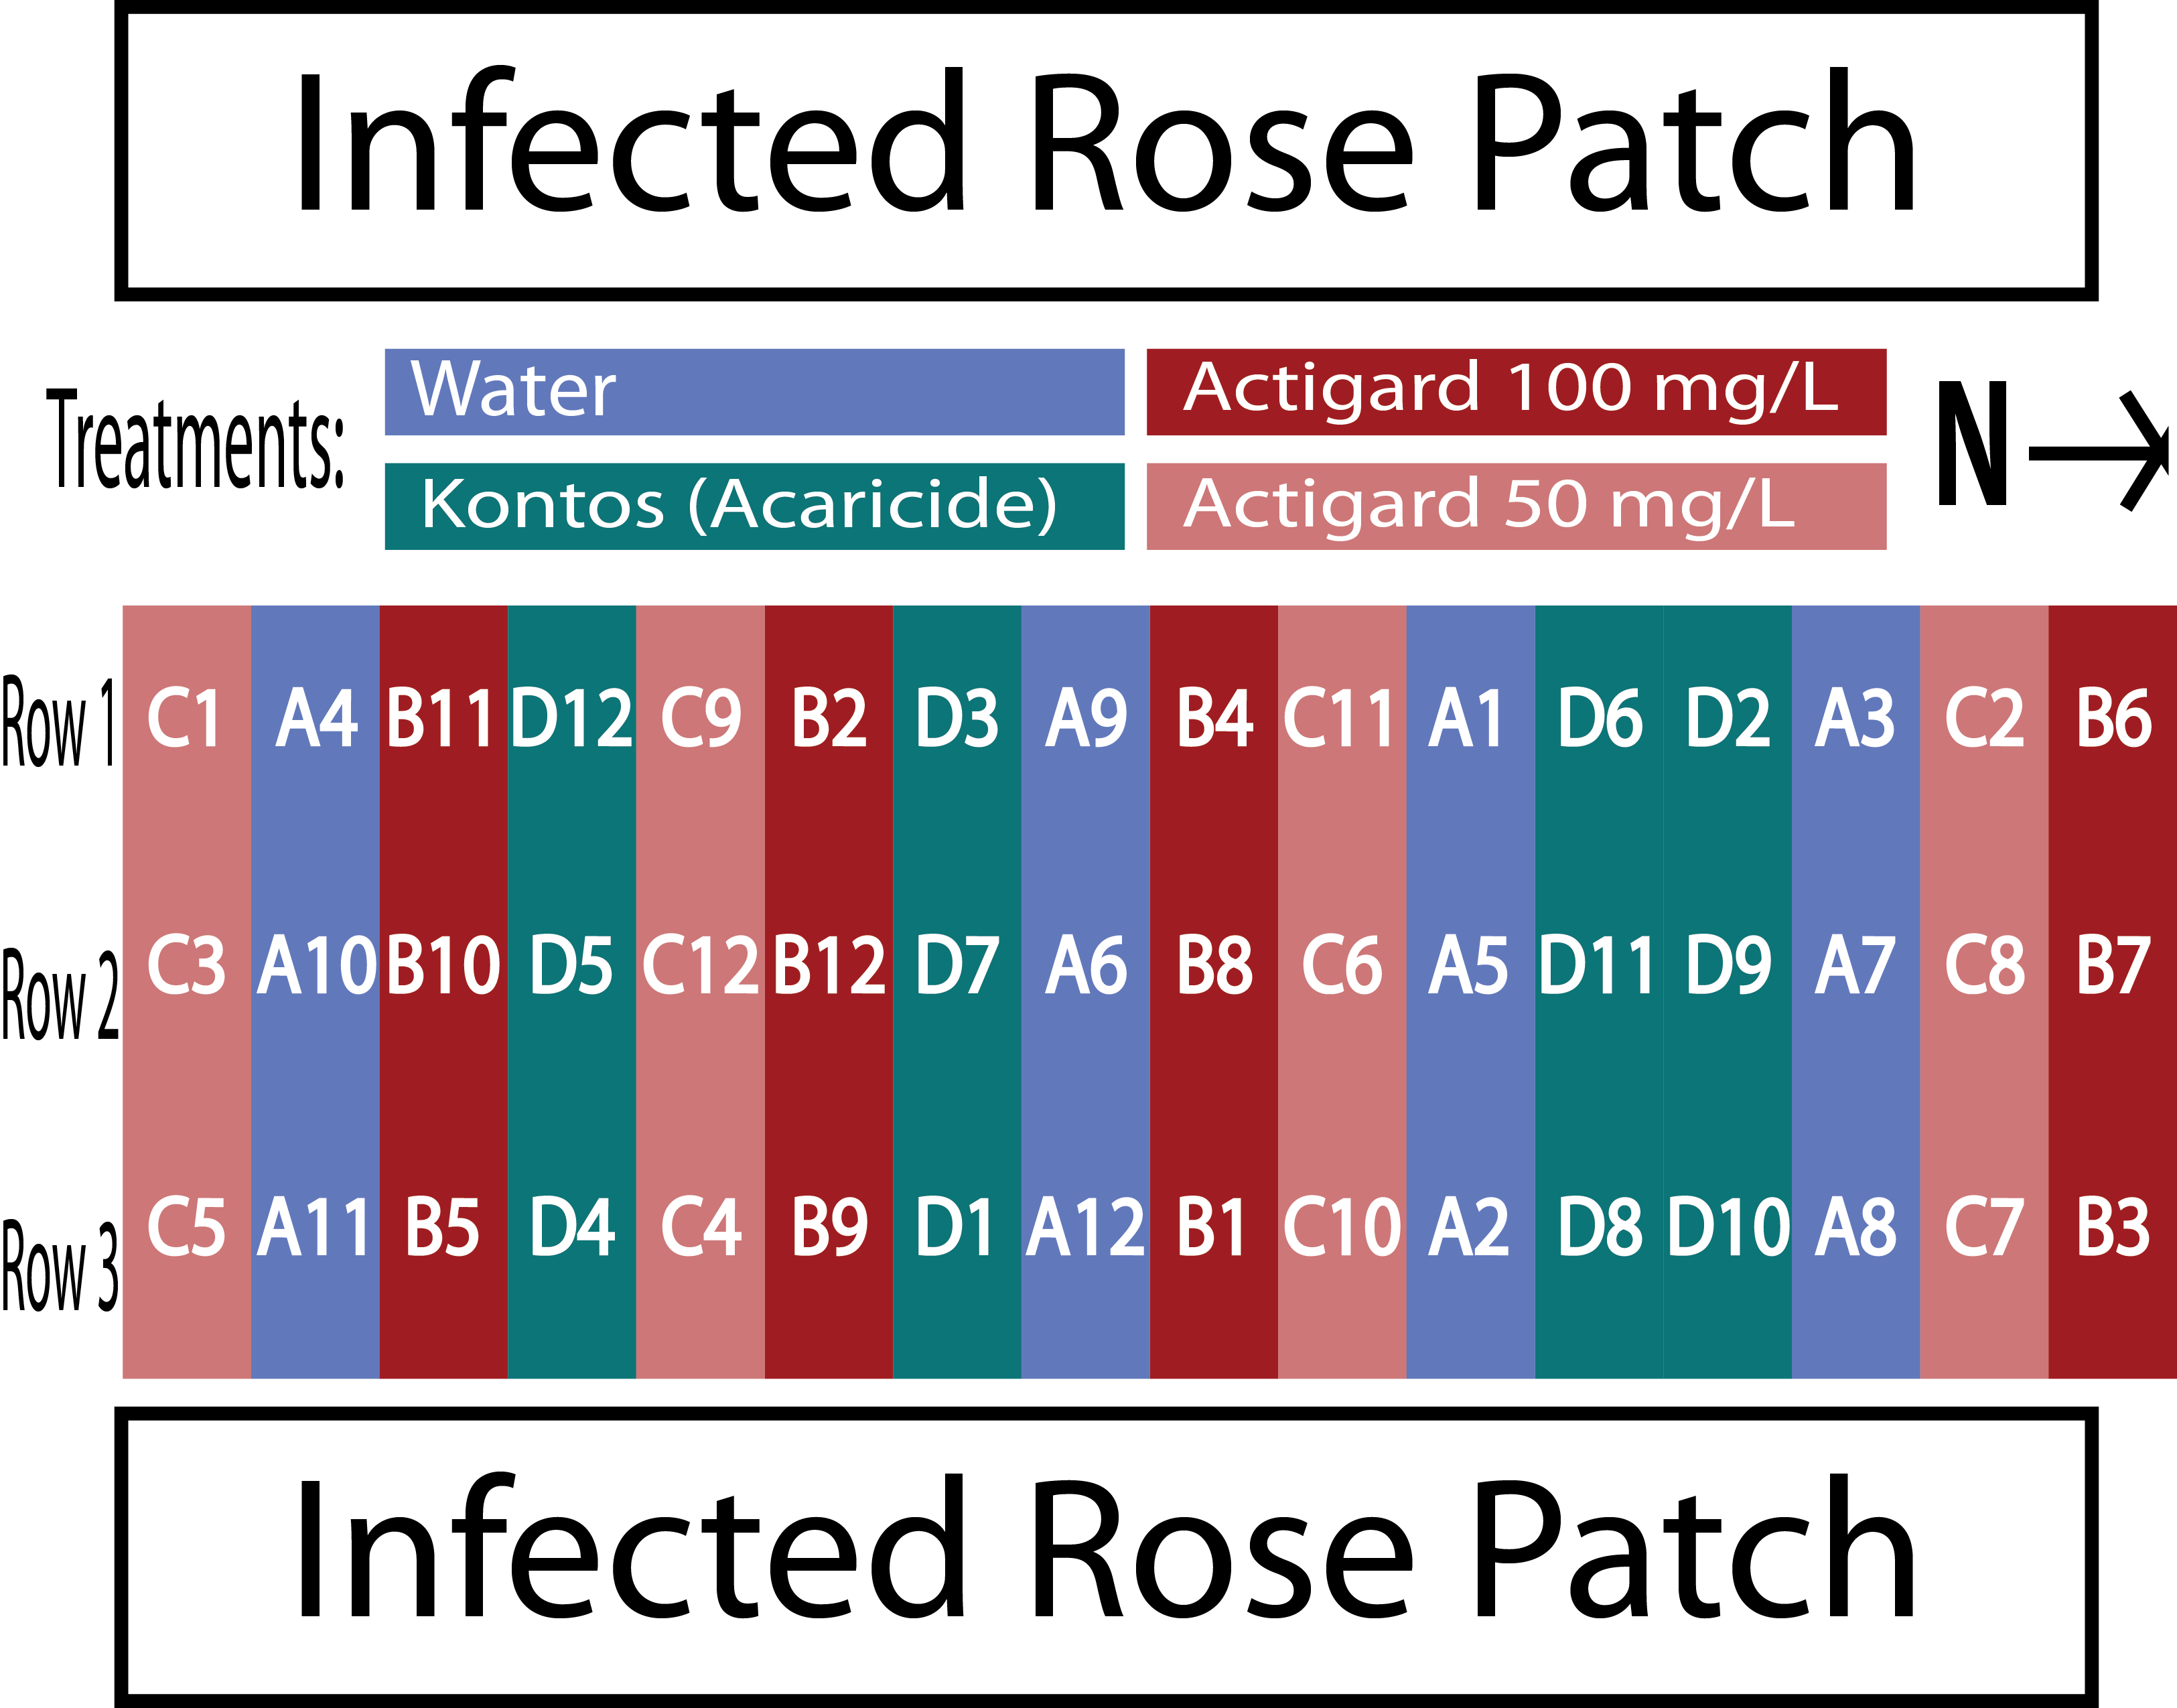
\includegraphics[width=0.8\linewidth]{figure/rrv_asm_plot_2019_griffin} \caption{Field design for testing the potential of Acibenzolar-S-Methyl to reduce populations of \textit{P. fructiphilus} by inducing Systemic Acquired Resistance in Pink Double Knock Out® roses. Trials were conducted for three months from September to December 2019 in Griffin, GA. Four treatments were applied weekly fo 12 weeks: Blue = Water Red = Actigard50WG 100 \si{\milli\gram}/L (High rate),  Pink = Actigard50WG 100 \si{\milli\gram}/L (Half rate) Turquoise = Kontos (Label rate). Flower cuttings were be taken weekly to record \textit{P. fructiphilus} numbers.}\label{fig:unnamed-chunk-2}
\end{figure}
\end{block}

\begin{block}{Data Collection: IPM}
\protect\hypertarget{data-collection-ipm}{}
\begin{itemize}
\tightlist
\item
  Cuttings taken weekly from six treated roses
\item
  Three flowers (buds if no flowers present)
\item
  \textasciitilde18 flowers/buds per bottle for each plot
\item
  Bottles with 95\% EtOH
\item
  Sieves to separate mites from the plant tissues.
\item
  Plant tissues dried \textasciitilde48 hrs at 50 °C, weighed
\item
  \emph{A. swirskii} applied on the 1st, 5th and 9th week
\end{itemize}
\end{block}

\begin{block}{Treatments: IPM}
\protect\hypertarget{treatments-ipm}{}
\begin{itemize}
\tightlist
\item
  Water - Control
\item
  Actigard - 100 mg/L
\item
  Ninja - label rate
\item
  Kontos - label rate
\item
  \emph{A. swirskii} (one sachet per rose treated)
\item
  \emph{A. swirskii} + Ninja (one sachet per rose treated, label rate)
\end{itemize}
\end{block}

\begin{block}{Plot Design: IPM - Athens}
\protect\hypertarget{plot-design-ipm---athens}{}
\begin{figure}
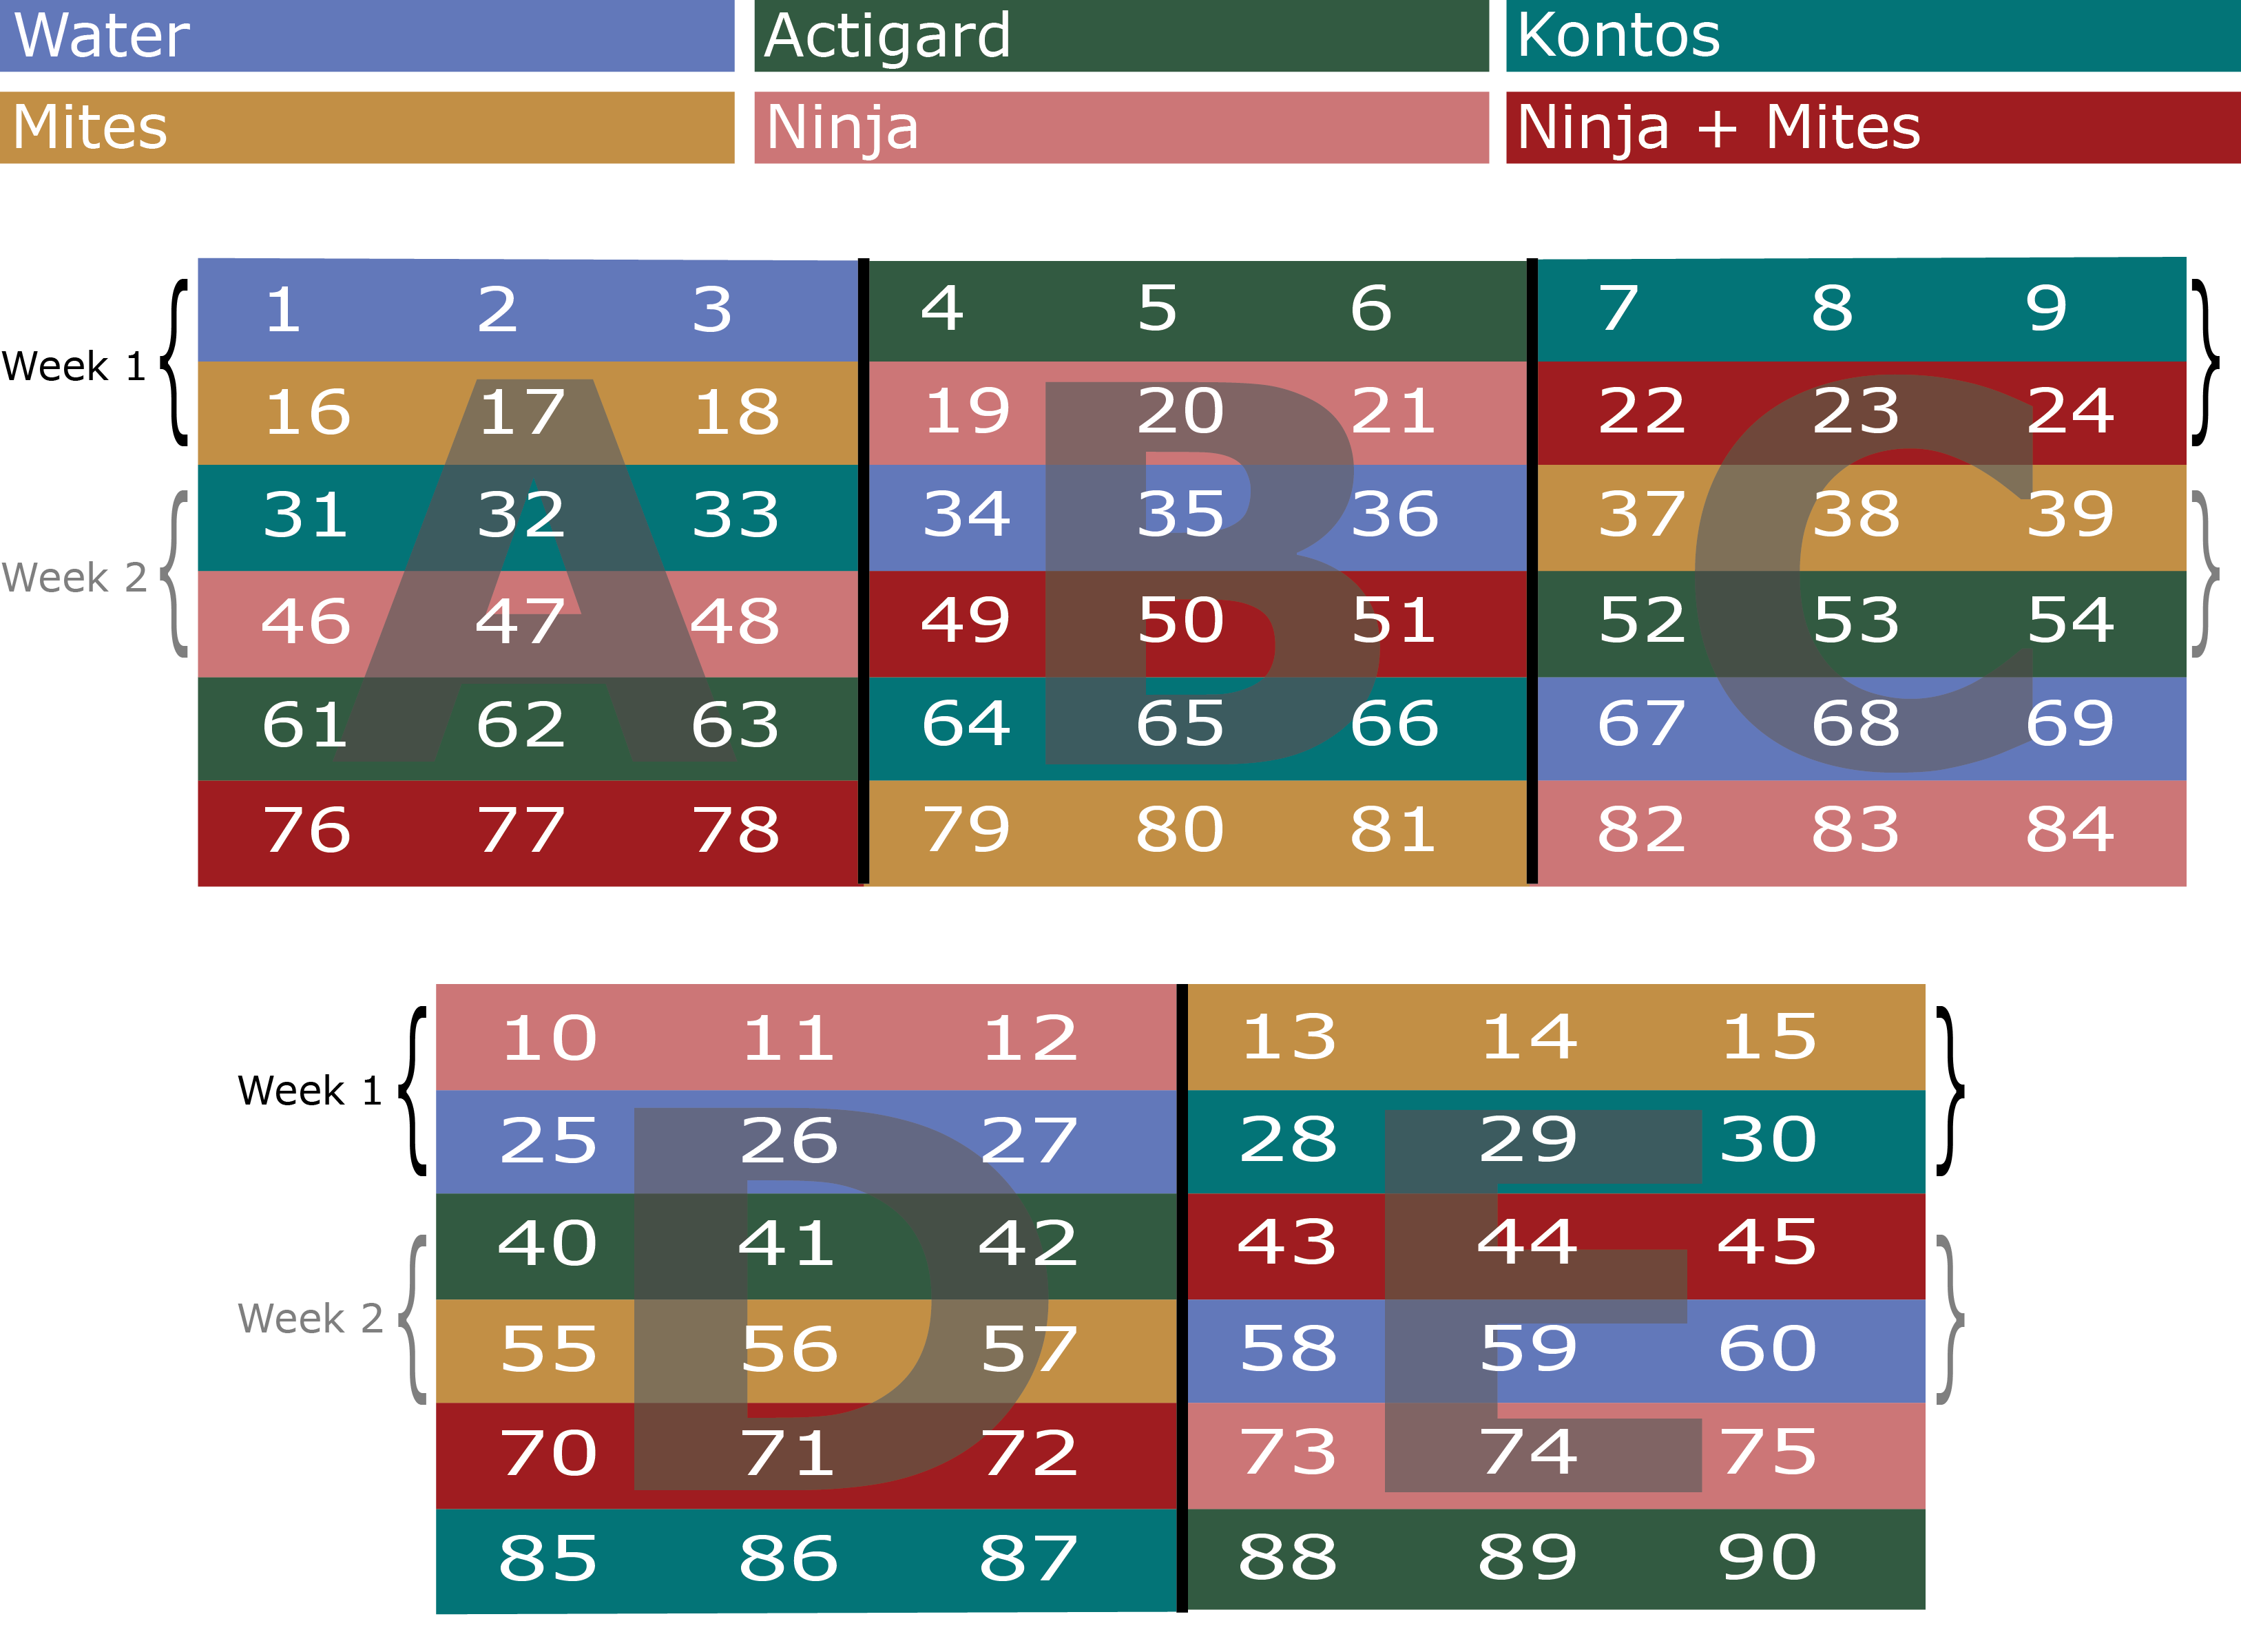
\includegraphics[width=0.8\linewidth]{figure/rrv_ipm_plot_map_2019_athens} \caption{Field design for Integrated Pest Management trials on Pink Double Knock Out® roses to control \textit{P. fructiphilus} in Athens, GA with five treatments. W = Water A = Actigard50WG, K = Kontos, M = \textit{A. swirkii} predatory mite sachets, N = SP2700 (Trade name: Ninja, SePro), + = \textit{A. swirskii} + Ninja combined treatments. All products were applied at their label rates for 12 weeks. Flower cuttings were taken weekly to record \textit{P. fructiphilus} numbers.}\label{fig:ipm-athens}
\end{figure}
\end{block}

\begin{block}{Plot Design: IPM - Griffin}
\protect\hypertarget{plot-design-ipm---griffin}{}
\begin{figure}
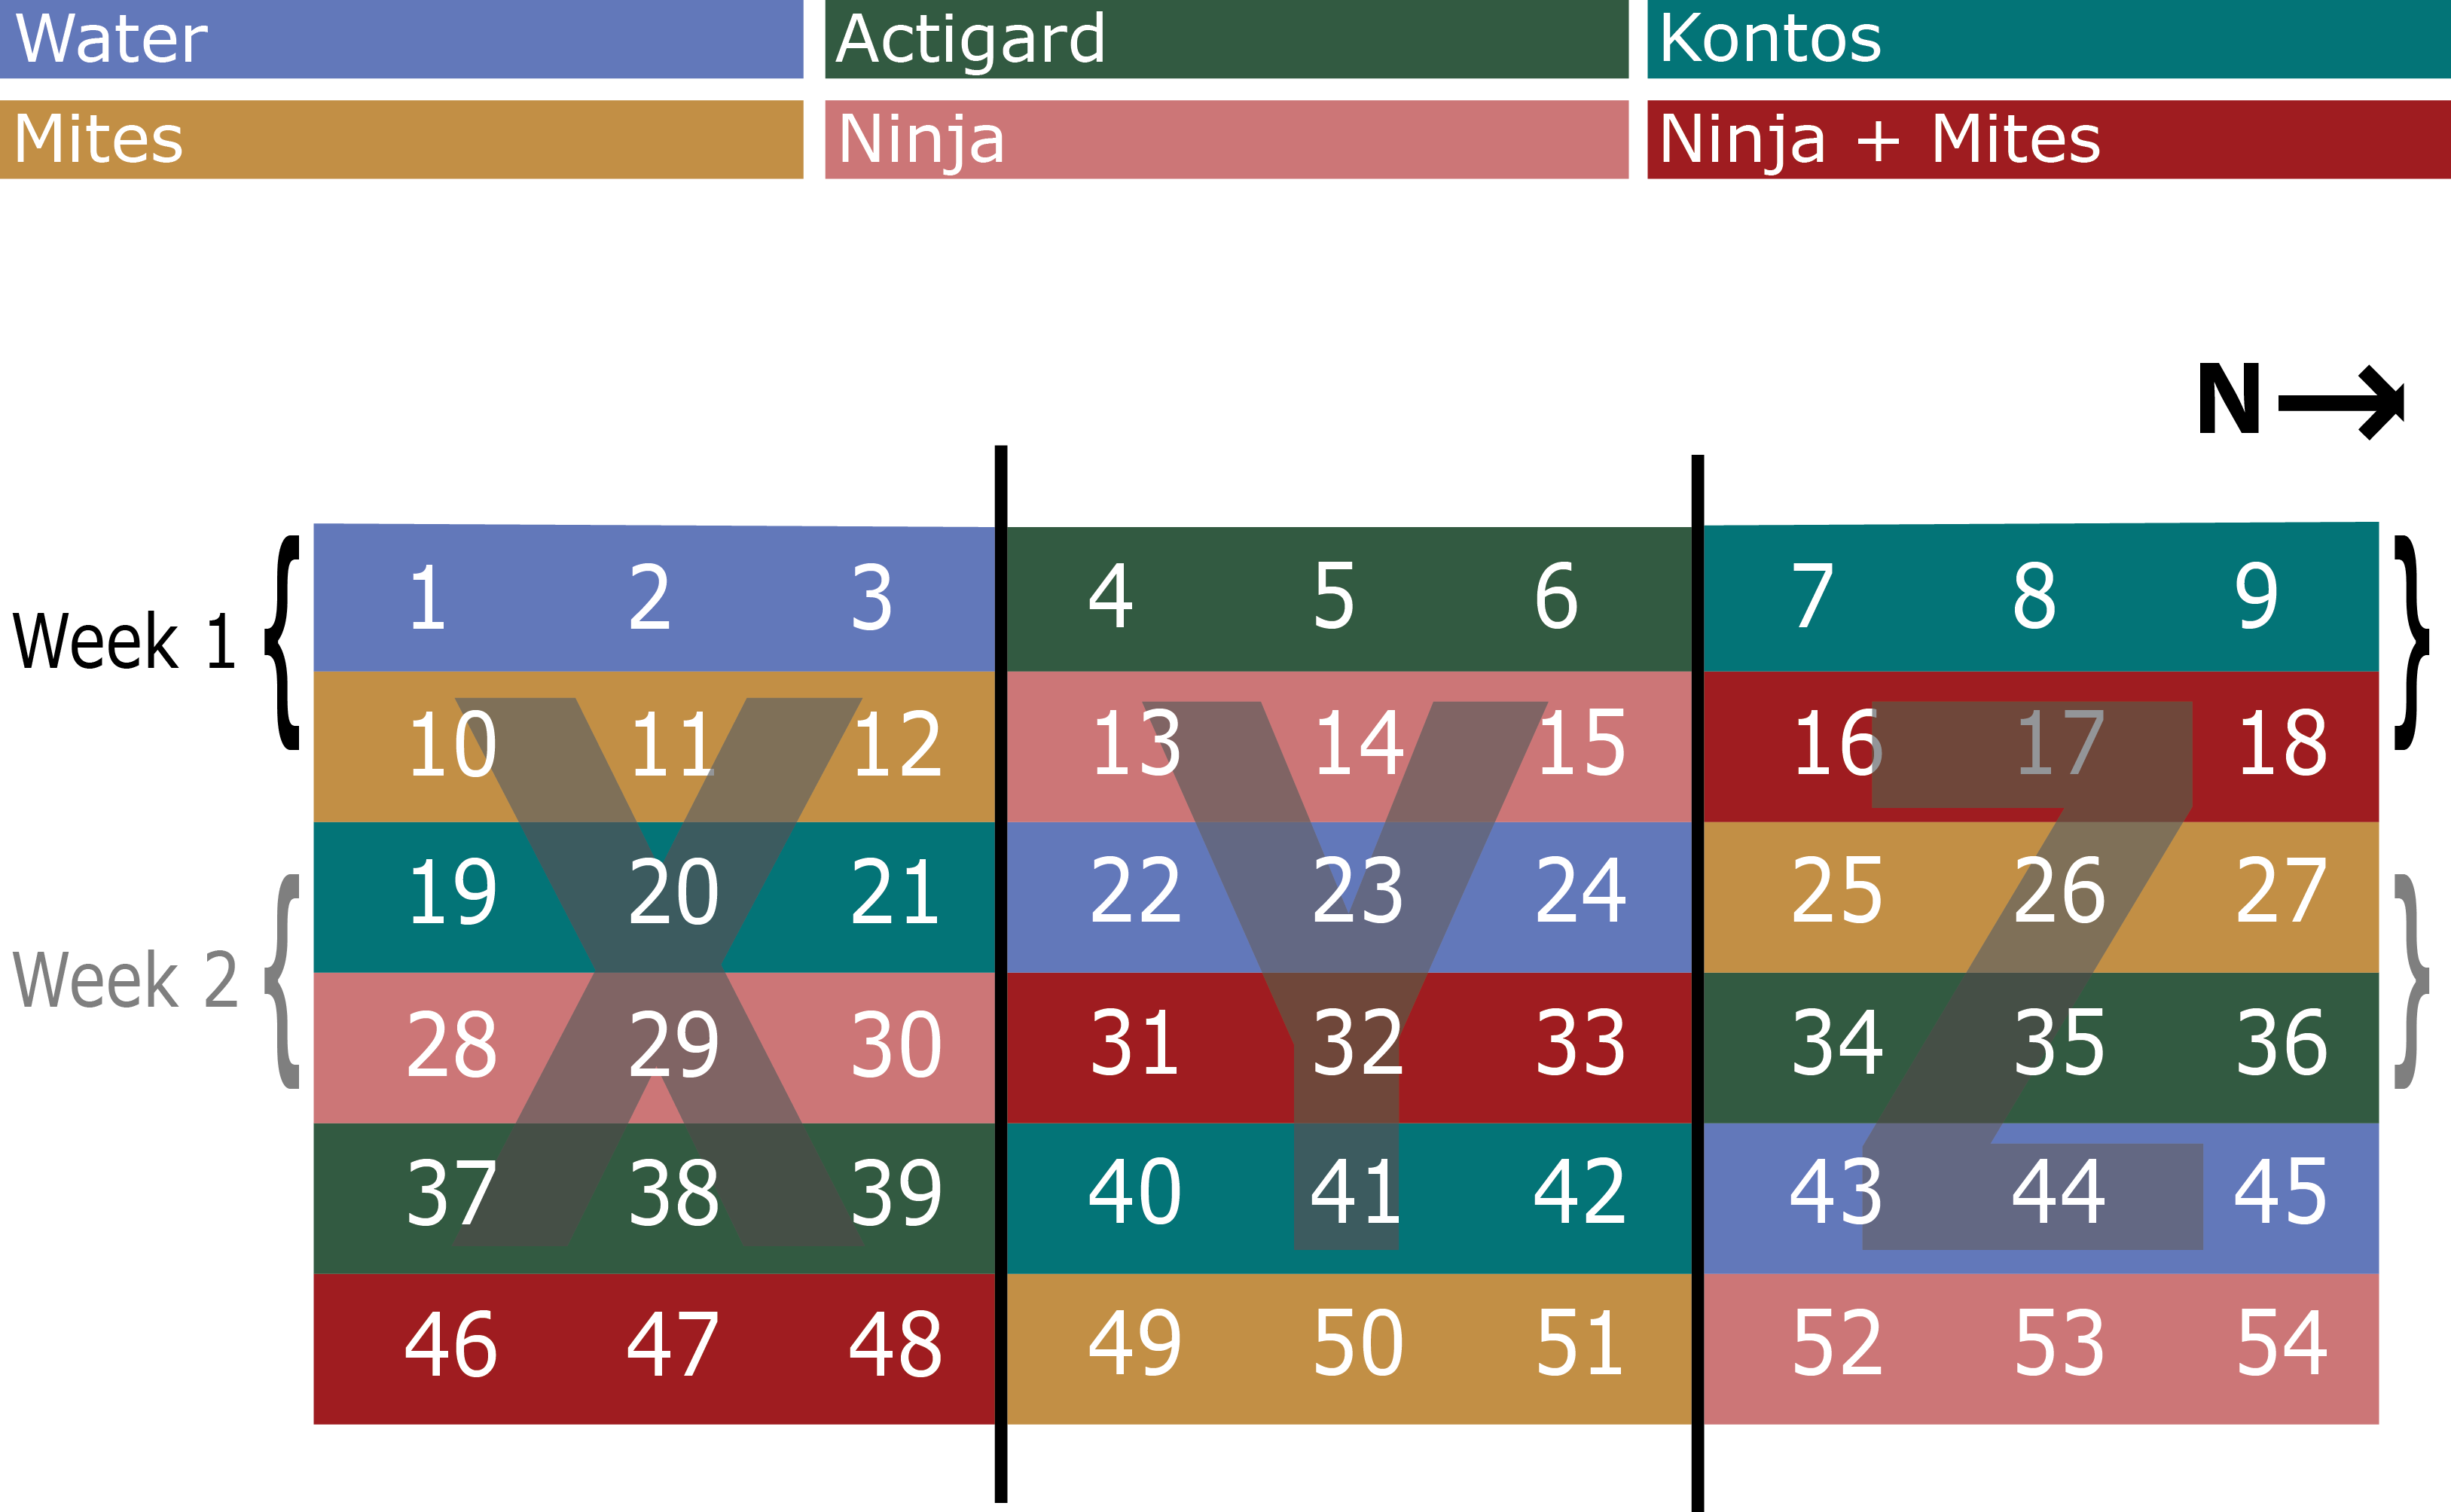
\includegraphics[width=0.8\linewidth]{figure/rrv_ipm_plot_map_2019_griffin} \caption{Field design for Integrated Pest Management trials on Pink Double Knock Out® roses to control \textit{P. fructiphilus} in Griffin, GA with five treatments. W = Water A = Actigard50WG, K = Kontos, M = \textit{A. swirkii} predatory mite sachets, N = SP2700 (Trade name: Ninja, SePro), + = \textit{A. swirskii} + Ninja combined treatments. All products were applied at their label rates for 12 weeks. Flower cuttings were taken weekly to record \textit{P. fructiphilus} numbers.}\label{fig:ipm-griff}
\end{figure}
\end{block}

\begin{block}{Plot Design: IPM - Tallahassee}
\protect\hypertarget{plot-design-ipm---tallahassee}{}
\begin{figure}
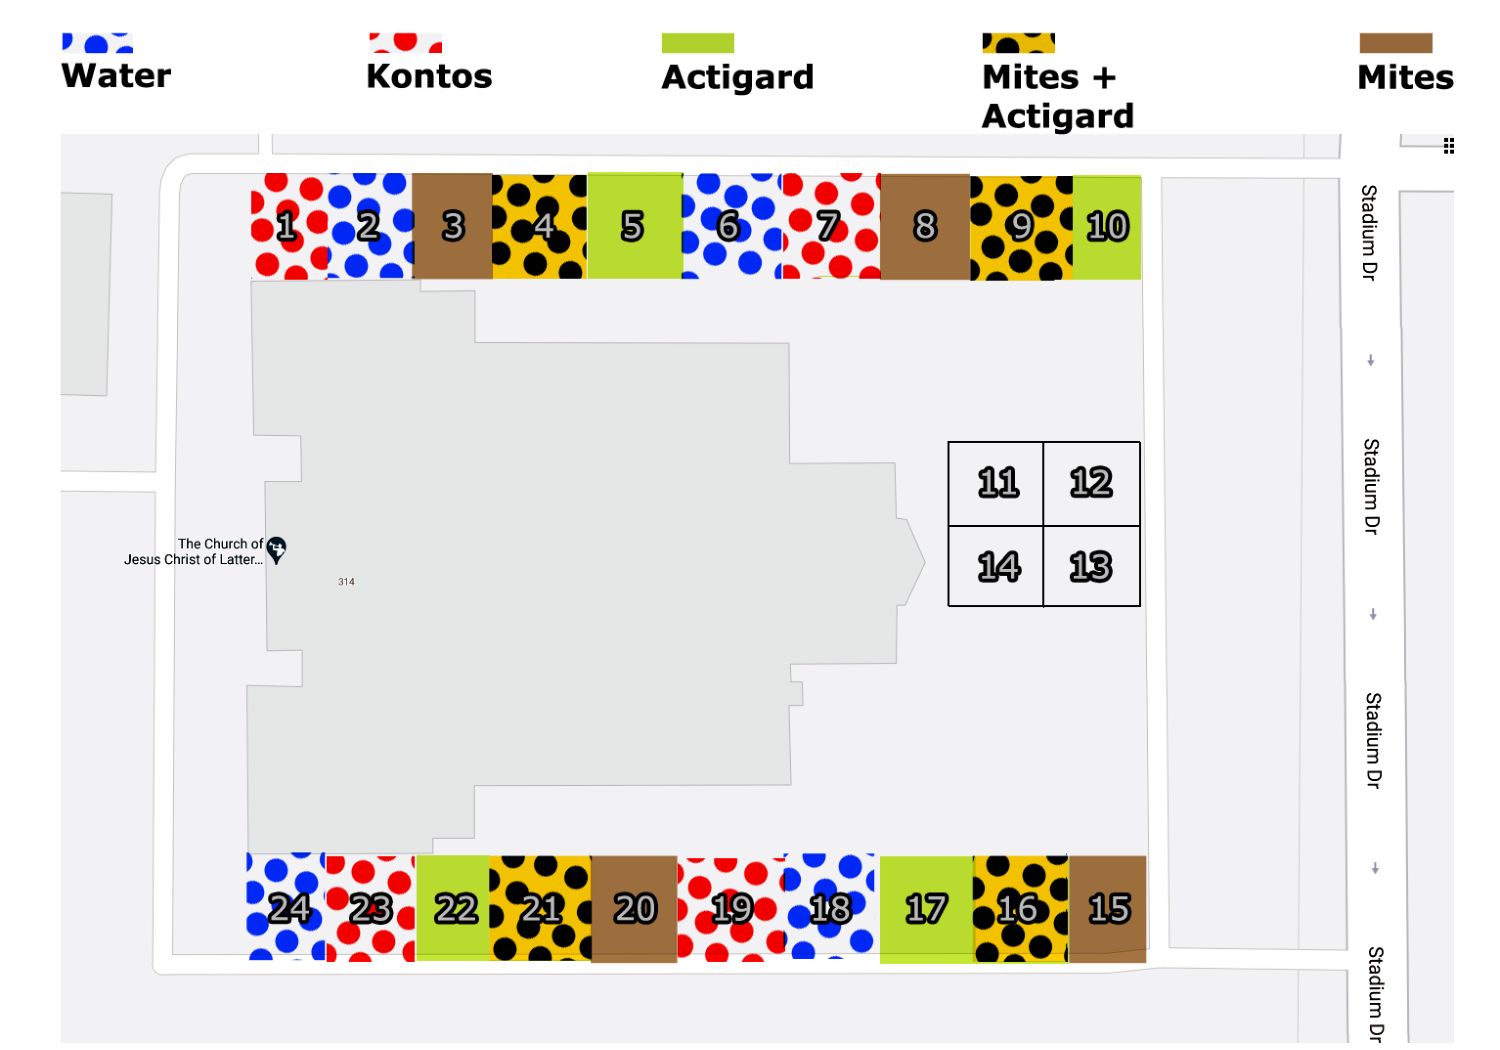
\includegraphics[width=0.8\linewidth]{asa-presentation-2021-denver_files/figure-beamer/unnamed-chunk-3-1} \caption{Field design for Integrated Pest Management trials on Pink Double Knock Out® roses to control \textit{P. fructiphilus} in Tallahassee, FL with five treatments: Water, Actigard50WG, Kontos, \textit{Amblyseius swirkii} predatory mite sachets, and \textit{A. swirskii} + Actigard combined treatments. All products were applied at their label rates for 12 weeks. Flower cuttings were taken weekly to record \textit{P. fructiphilus} numbers.}\label{fig:unnamed-chunk-3}
\end{figure}
\end{block}
\end{frame}

\begin{frame}{Results}
\protect\hypertarget{results-asm-ipm}{}
Combining predatory mites with a SAR-inducer was as effective as the
miticide alone, and controlled herbivorous mite populations more than
either SAR-induction or predatory mites alone

\begin{figure}
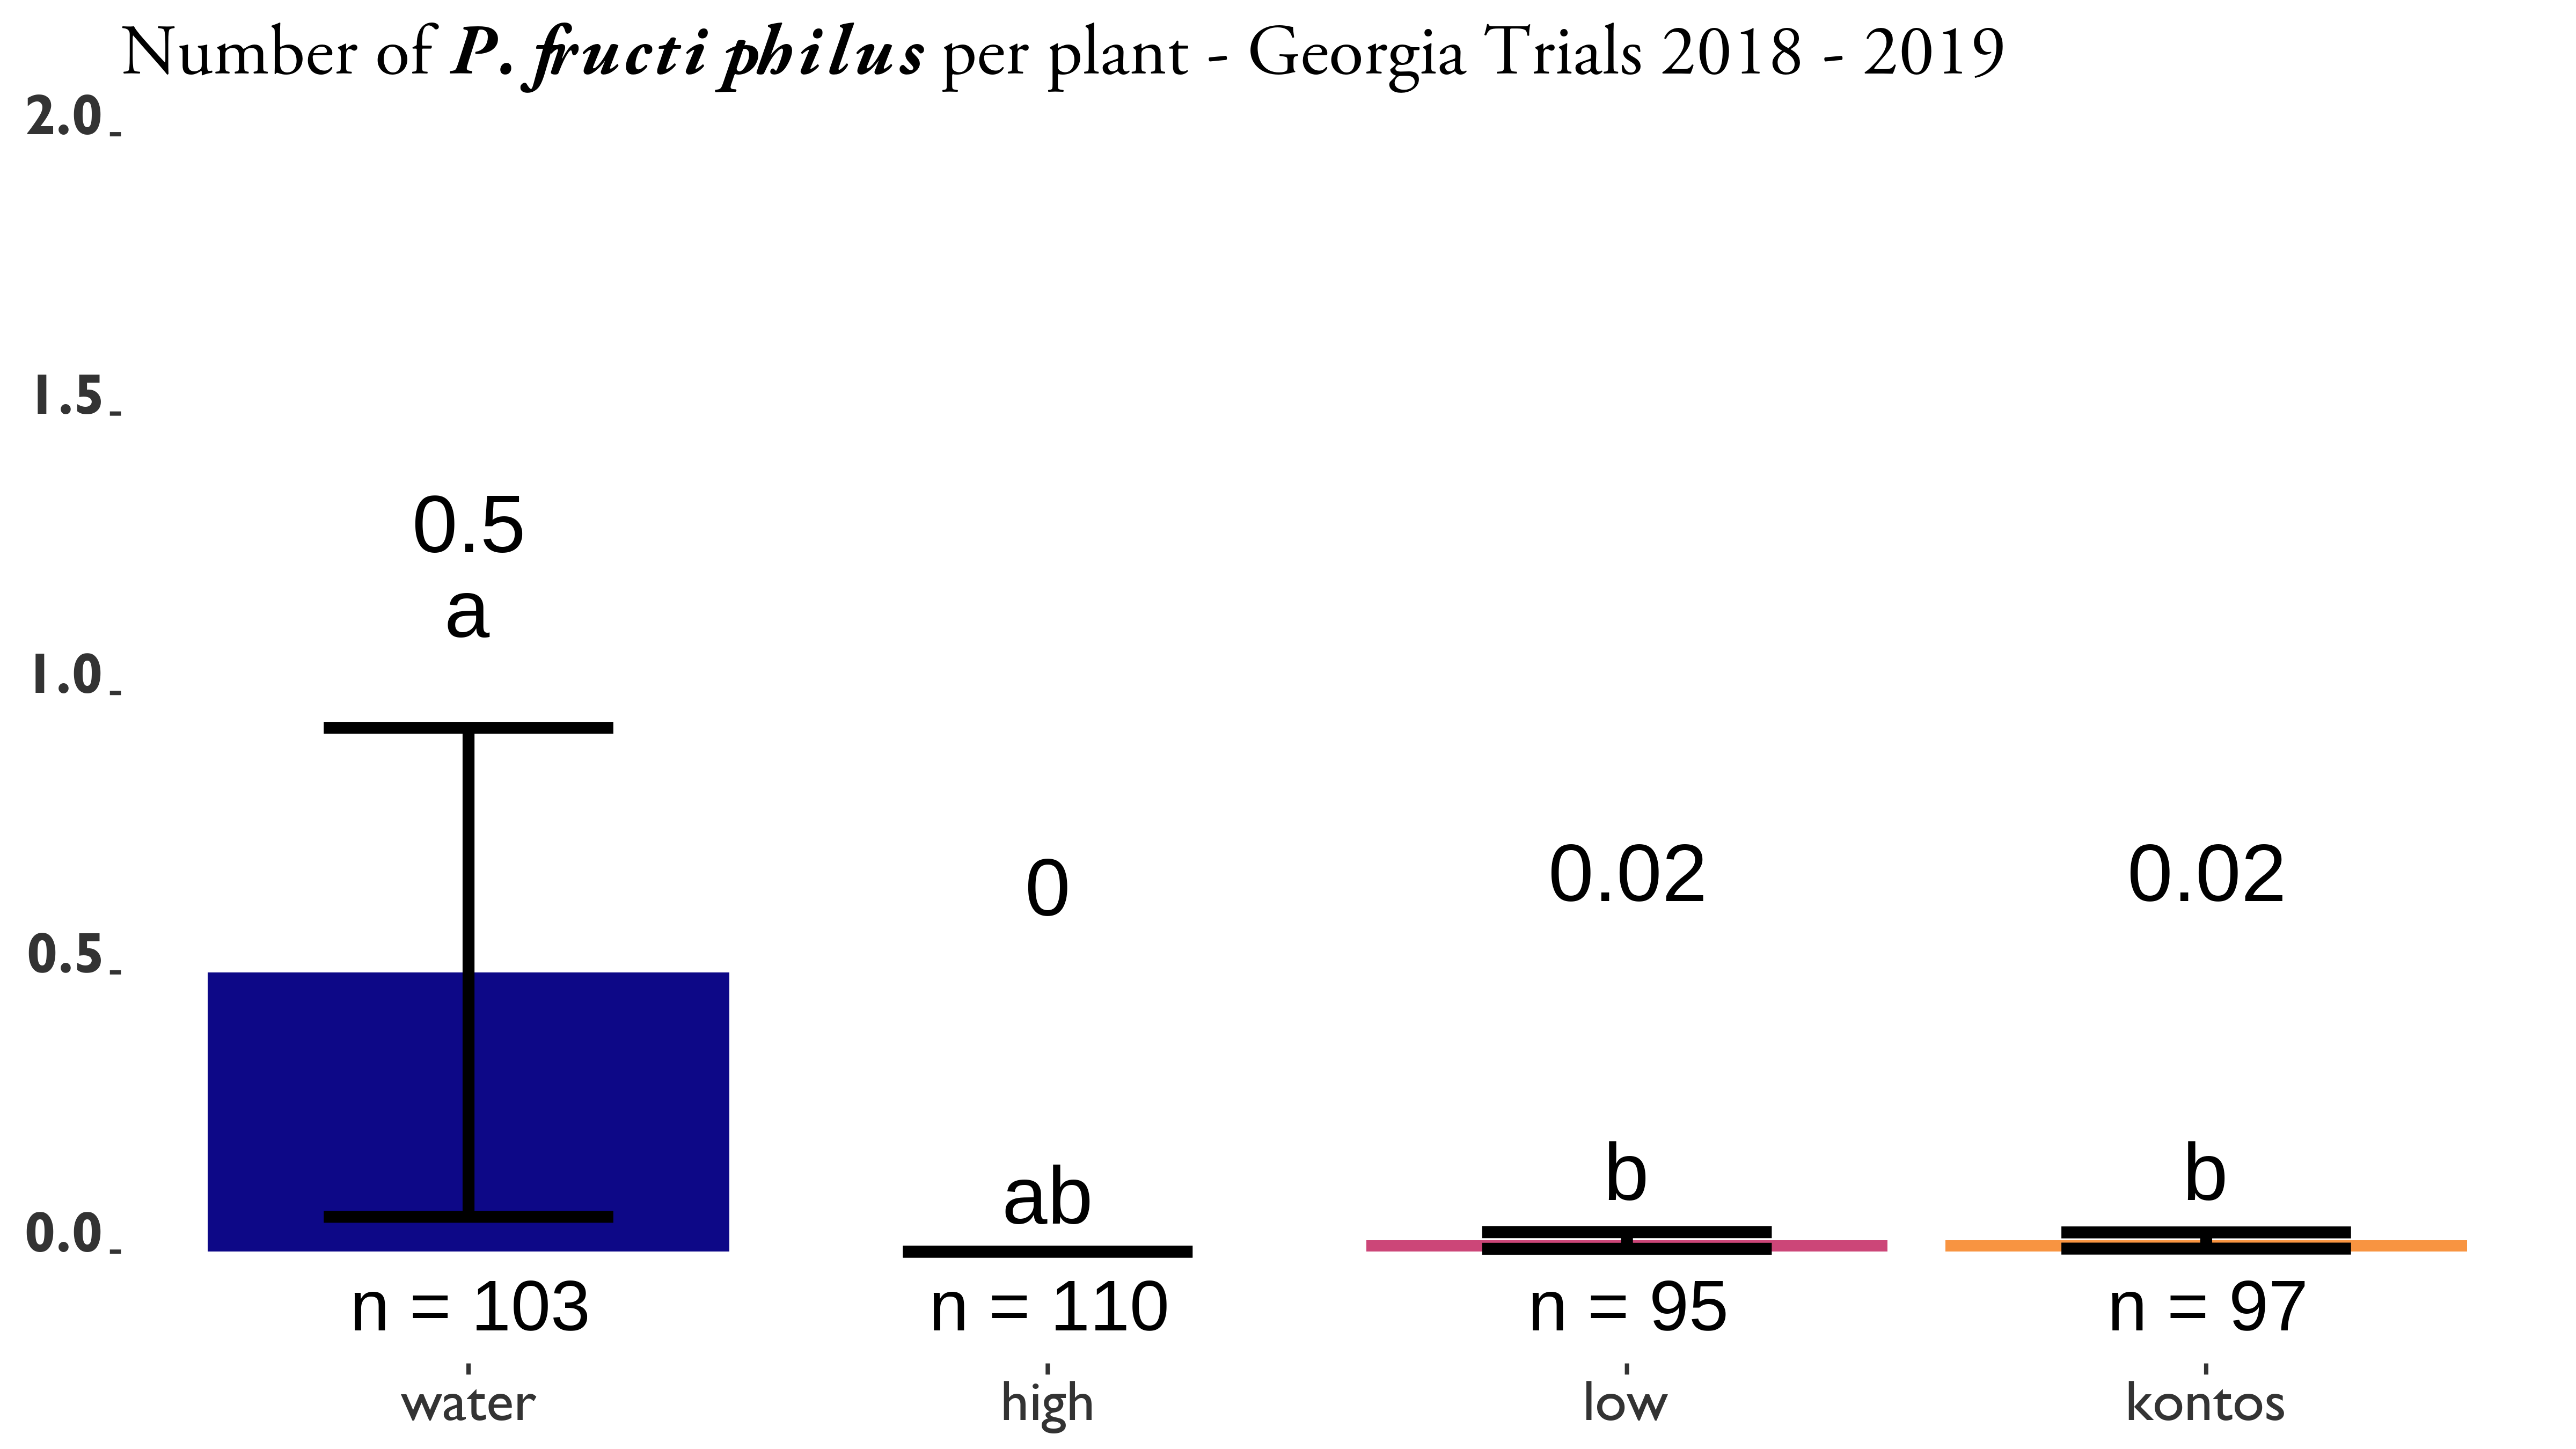
\includegraphics[width=0.8\linewidth]{figure/actigard_graph} \caption{SAR-induction trials on Pink Double Knock Out® roses to control \textit{Phyllocoptes fructiphilus} in Athens and Griffin, GA. Statistical significance was determined using Tukey contrasts for multiple Comparisons of means. Groups which share letters are not statistically different from one another. $\alpha = 0.05$. water = Water Control, High = 100 \si{\milli\gram}/\si{\liter} Actigard® 50WG (Syngenta, Greensboro, NC, USA) acibenzolar-S-methyl (ASM), low = 50 \si{\milli\gram}/\si{\liter} Actigard® 50WG (Syngenta, Greensboro, NC, USA) acibenzolar-S-methyl (ASM), kontos = Kontos® Miticide Insecticide - Spirotetramat (Bayer Corporation, Whippany, New Jersey, USA), untreated = No treatment. All products were applied for 12 weeks. Flower cuttings were taken weekly to record the numbers of herbivorous mites.}\label{fig:asm-graph}
\end{figure}

\begin{block}{ASM Trial: Athens 2018}
\protect\hypertarget{asm-trial-athens-2018}{}
\begin{table}

\caption{\label{tab:asm-athns-2018-table}Progression of RRD on SAR-induced Pink Double Knock Out® roses in Athens, GA 2018.}
\centering
\resizebox{\linewidth}{!}{
\begin{tabular}[t]{lllrrrrrrrrrrrrrrr}
\toprule
Plant & Treatment & RRD & P.fructiphilus & Other Mites & Week 1 & Week 2 & Week 3 & Week 4 & Week 5 & Week 6 & Week 7 & Week 8 & Week 9 & Week 10 & Week 17 & AUDPC & Final disease severity (\%)\\
\midrule
\cellcolor{gray!6}{W1} & \cellcolor{gray!6}{Water} & \cellcolor{gray!6}{S} & \cellcolor{gray!6}{2} & \cellcolor{gray!6}{0} & \cellcolor{gray!6}{0} & \cellcolor{gray!6}{0} & \cellcolor{gray!6}{0} & \cellcolor{gray!6}{0.0} & \cellcolor{gray!6}{0.0} & \cellcolor{gray!6}{0.0} & \cellcolor{gray!6}{1.5} & \cellcolor{gray!6}{1.5} & \cellcolor{gray!6}{4.5} & \cellcolor{gray!6}{1.5} & \cellcolor{gray!6}{17.5} & \cellcolor{gray!6}{124.25} & \cellcolor{gray!6}{17.5}\\
W2 & Water & A? & 0 & 0 & 0 & 0 & 0 & 0.0 & 0.0 & 0.0 & 0.0 & 1.5 & 4.5 & 1.5 & 0.0 & 52.50 & 0.0\\
\cellcolor{gray!6}{W3} & \cellcolor{gray!6}{Water} & \cellcolor{gray!6}{A} & \cellcolor{gray!6}{0} & \cellcolor{gray!6}{0} & \cellcolor{gray!6}{0} & \cellcolor{gray!6}{0} & \cellcolor{gray!6}{0} & \cellcolor{gray!6}{0.0} & \cellcolor{gray!6}{0.0} & \cellcolor{gray!6}{0.0} & \cellcolor{gray!6}{0.0} & \cellcolor{gray!6}{1.5} & \cellcolor{gray!6}{4.5} & \cellcolor{gray!6}{1.5} & \cellcolor{gray!6}{1.5} & \cellcolor{gray!6}{57.75} & \cellcolor{gray!6}{1.5}\\
W4 & Water & A & 0 & 0 & 0 & 0 & 0 & 0.0 & 0.0 & 0.0 & 1.5 & 1.5 & 0.0 & 1.5 & 0.0 & 31.50 & 0.0\\
\cellcolor{gray!6}{W5} & \cellcolor{gray!6}{Water} & \cellcolor{gray!6}{S} & \cellcolor{gray!6}{0} & \cellcolor{gray!6}{0} & \cellcolor{gray!6}{0} & \cellcolor{gray!6}{0} & \cellcolor{gray!6}{0} & \cellcolor{gray!6}{0.0} & \cellcolor{gray!6}{0.0} & \cellcolor{gray!6}{0.0} & \cellcolor{gray!6}{1.5} & \cellcolor{gray!6}{1.5} & \cellcolor{gray!6}{0.0} & \cellcolor{gray!6}{0.0} & \cellcolor{gray!6}{9.0} & \cellcolor{gray!6}{52.50} & \cellcolor{gray!6}{9.0}\\
\addlinespace
W6 & Water & S & 1 & 1 & 0 & 0 & 0 & 0.0 & 0.0 & 0.0 & 1.5 & 1.5 & 1.5 & 1.5 & 9.0 & 73.50 & 9.0\\
\cellcolor{gray!6}{W7} & \cellcolor{gray!6}{Water} & \cellcolor{gray!6}{A} & \cellcolor{gray!6}{0} & \cellcolor{gray!6}{0} & \cellcolor{gray!6}{0} & \cellcolor{gray!6}{0} & \cellcolor{gray!6}{0} & \cellcolor{gray!6}{0.0} & \cellcolor{gray!6}{0.0} & \cellcolor{gray!6}{0.0} & \cellcolor{gray!6}{0.0} & \cellcolor{gray!6}{0.0} & \cellcolor{gray!6}{1.5} & \cellcolor{gray!6}{1.5} & \cellcolor{gray!6}{1.5} & \cellcolor{gray!6}{26.25} & \cellcolor{gray!6}{1.5}\\
W8 & Water & A? & 0 & 0 & 0 & 0 & 0 & 0.0 & 0.0 & 0.0 & 0.0 & 0.0 & 1.5 & 1.5 & 4.5 & 36.75 & 4.5\\
\cellcolor{gray!6}{W9} & \cellcolor{gray!6}{Water} & \cellcolor{gray!6}{A} & \cellcolor{gray!6}{0} & \cellcolor{gray!6}{0} & \cellcolor{gray!6}{0} & \cellcolor{gray!6}{0} & \cellcolor{gray!6}{0} & \cellcolor{gray!6}{0.0} & \cellcolor{gray!6}{0.0} & \cellcolor{gray!6}{0.0} & \cellcolor{gray!6}{1.5} & \cellcolor{gray!6}{1.5} & \cellcolor{gray!6}{1.5} & \cellcolor{gray!6}{1.5} & \cellcolor{gray!6}{0.0} & \cellcolor{gray!6}{42.00} & \cellcolor{gray!6}{0.0}\\
W10 & Water & A? & 0 & 0 & 0 & 0 & 0 & 0.0 & 0.0 & 0.0 & 0.0 & 1.5 & 1.5 & 1.5 & 0.0 & 31.50 & 0.0\\
\addlinespace
\cellcolor{gray!6}{W11} & \cellcolor{gray!6}{Water} & \cellcolor{gray!6}{A?} & \cellcolor{gray!6}{0} & \cellcolor{gray!6}{0} & \cellcolor{gray!6}{0} & \cellcolor{gray!6}{0} & \cellcolor{gray!6}{0} & \cellcolor{gray!6}{0.0} & \cellcolor{gray!6}{0.0} & \cellcolor{gray!6}{1.5} & \cellcolor{gray!6}{0.0} & \cellcolor{gray!6}{0.0} & \cellcolor{gray!6}{1.5} & \cellcolor{gray!6}{1.5} & \cellcolor{gray!6}{1.5} & \cellcolor{gray!6}{36.75} & \cellcolor{gray!6}{1.5}\\
W12 & Water & S & 0 & 1 & 0 & 0 & 0 & 0.0 & 0.0 & 0.0 & 1.5 & 1.5 & 1.5 & 1.5 & 17.5 & 103.25 & 17.5\\
\cellcolor{gray!6}{L1} & \cellcolor{gray!6}{Low} & \cellcolor{gray!6}{A} & \cellcolor{gray!6}{0} & \cellcolor{gray!6}{0} & \cellcolor{gray!6}{0} & \cellcolor{gray!6}{0} & \cellcolor{gray!6}{0} & \cellcolor{gray!6}{0.0} & \cellcolor{gray!6}{0.0} & \cellcolor{gray!6}{0.0} & \cellcolor{gray!6}{0.0} & \cellcolor{gray!6}{1.5} & \cellcolor{gray!6}{4.5} & \cellcolor{gray!6}{1.5} & \cellcolor{gray!6}{0.0} & \cellcolor{gray!6}{52.50} & \cellcolor{gray!6}{0.0}\\
L2 & Low & A & 0 & 0 & 0 & 0 & 0 & 0.0 & 0.0 & 0.0 & 0.0 & 0.0 & 1.5 & 1.5 & 4.5 & 36.75 & 4.5\\
\cellcolor{gray!6}{L3} & \cellcolor{gray!6}{Low} & \cellcolor{gray!6}{S} & \cellcolor{gray!6}{0} & \cellcolor{gray!6}{0} & \cellcolor{gray!6}{0} & \cellcolor{gray!6}{0} & \cellcolor{gray!6}{0} & \cellcolor{gray!6}{0.0} & \cellcolor{gray!6}{0.0} & \cellcolor{gray!6}{0.0} & \cellcolor{gray!6}{4.5} & \cellcolor{gray!6}{1.5} & \cellcolor{gray!6}{4.5} & \cellcolor{gray!6}{0.0} & \cellcolor{gray!6}{1.5} & \cellcolor{gray!6}{78.75} & \cellcolor{gray!6}{1.5}\\
\addlinespace
L4 & Low & A & 0 & 0 & 0 & 0 & 0 & 0.0 & 0.0 & 1.5 & 1.5 & 1.5 & 0.0 & 0.0 & 1.5 & 36.75 & 1.5\\
\cellcolor{gray!6}{L5} & \cellcolor{gray!6}{Low} & \cellcolor{gray!6}{S} & \cellcolor{gray!6}{0} & \cellcolor{gray!6}{0} & \cellcolor{gray!6}{0} & \cellcolor{gray!6}{0} & \cellcolor{gray!6}{0} & \cellcolor{gray!6}{0.0} & \cellcolor{gray!6}{0.0} & \cellcolor{gray!6}{1.5} & \cellcolor{gray!6}{0.0} & \cellcolor{gray!6}{1.5} & \cellcolor{gray!6}{0.0} & \cellcolor{gray!6}{0.0} & \cellcolor{gray!6}{17.5} & \cellcolor{gray!6}{82.25} & \cellcolor{gray!6}{17.5}\\
L6 & Low & A & 0 & 0 & 0 & 0 & 0 & 0.0 & 0.0 & 0.0 & 0.0 & 0.0 & 0.0 & 1.5 & 9.0 & 42.00 & 9.0\\
\cellcolor{gray!6}{L7} & \cellcolor{gray!6}{Low} & \cellcolor{gray!6}{S} & \cellcolor{gray!6}{0} & \cellcolor{gray!6}{0} & \cellcolor{gray!6}{0} & \cellcolor{gray!6}{0} & \cellcolor{gray!6}{0} & \cellcolor{gray!6}{1.5} & \cellcolor{gray!6}{1.5} & \cellcolor{gray!6}{1.5} & \cellcolor{gray!6}{0.0} & \cellcolor{gray!6}{0.0} & \cellcolor{gray!6}{1.5} & \cellcolor{gray!6}{1.5} & \cellcolor{gray!6}{17.5} & \cellcolor{gray!6}{113.75} & \cellcolor{gray!6}{17.5}\\
L8 & Low & A & 0 & 0 & 0 & 0 & 0 & 0.0 & 1.5 & 1.5 & 4.5 & 1.5 & 1.5 & 1.5 & 4.5 & 99.75 & 4.5\\
\addlinespace
\cellcolor{gray!6}{L9} & \cellcolor{gray!6}{Low} & \cellcolor{gray!6}{S} & \cellcolor{gray!6}{0} & \cellcolor{gray!6}{0} & \cellcolor{gray!6}{0} & \cellcolor{gray!6}{0} & \cellcolor{gray!6}{0} & \cellcolor{gray!6}{0.0} & \cellcolor{gray!6}{0.0} & \cellcolor{gray!6}{0.0} & \cellcolor{gray!6}{1.5} & \cellcolor{gray!6}{0.0} & \cellcolor{gray!6}{0.0} & \cellcolor{gray!6}{0.0} & \cellcolor{gray!6}{17.5} & \cellcolor{gray!6}{71.75} & \cellcolor{gray!6}{17.5}\\
L10 & Low & A & 0 & 0 & 0 & 0 & 0 & 0.0 & 0.0 & 0.0 & 1.5 & 1.5 & 0.0 & 1.5 & 4.5 & 47.25 & 4.5\\
\cellcolor{gray!6}{L11} & \cellcolor{gray!6}{Low} & \cellcolor{gray!6}{A} & \cellcolor{gray!6}{0} & \cellcolor{gray!6}{0} & \cellcolor{gray!6}{0} & \cellcolor{gray!6}{0} & \cellcolor{gray!6}{0} & \cellcolor{gray!6}{0.0} & \cellcolor{gray!6}{0.0} & \cellcolor{gray!6}{0.0} & \cellcolor{gray!6}{0.0} & \cellcolor{gray!6}{1.5} & \cellcolor{gray!6}{4.5} & \cellcolor{gray!6}{1.5} & \cellcolor{gray!6}{0.0} & \cellcolor{gray!6}{52.50} & \cellcolor{gray!6}{0.0}\\
L12 & Low & A & 0 & 0 & 0 & 0 & 0 & 0.0 & 0.0 & 1.5 & 0.0 & 0.0 & 1.5 & 1.5 & 1.5 & 36.75 & 1.5\\
\cellcolor{gray!6}{H1} & \cellcolor{gray!6}{High} & \cellcolor{gray!6}{S?} & \cellcolor{gray!6}{0} & \cellcolor{gray!6}{0} & \cellcolor{gray!6}{0} & \cellcolor{gray!6}{0} & \cellcolor{gray!6}{0} & \cellcolor{gray!6}{0.0} & \cellcolor{gray!6}{0.0} & \cellcolor{gray!6}{0.0} & \cellcolor{gray!6}{1.5} & \cellcolor{gray!6}{0.0} & \cellcolor{gray!6}{4.5} & \cellcolor{gray!6}{4.5} & \cellcolor{gray!6}{1.5} & \cellcolor{gray!6}{78.75} & \cellcolor{gray!6}{1.5}\\
\addlinespace
H2 & High & S & 0 & 0 & 0 & 0 & 0 & 0.0 & 0.0 & 1.5 & 0.0 & 0.0 & 0.0 & 0.0 & 17.5 & 71.75 & 17.5\\
\cellcolor{gray!6}{H3} & \cellcolor{gray!6}{High} & \cellcolor{gray!6}{S} & \cellcolor{gray!6}{0} & \cellcolor{gray!6}{0} & \cellcolor{gray!6}{0} & \cellcolor{gray!6}{0} & \cellcolor{gray!6}{0} & \cellcolor{gray!6}{0.0} & \cellcolor{gray!6}{0.0} & \cellcolor{gray!6}{0.0} & \cellcolor{gray!6}{1.5} & \cellcolor{gray!6}{1.5} & \cellcolor{gray!6}{1.5} & \cellcolor{gray!6}{1.5} & \cellcolor{gray!6}{17.5} & \cellcolor{gray!6}{103.25} & \cellcolor{gray!6}{17.5}\\
H4 & High & A & 0 & 0 & 0 & 0 & 0 & 0.0 & 0.0 & 0.0 & 0.0 & 0.0 & 1.5 & 1.5 & 1.5 & 26.25 & 1.5\\
\cellcolor{gray!6}{H5} & \cellcolor{gray!6}{High} & \cellcolor{gray!6}{S} & \cellcolor{gray!6}{0} & \cellcolor{gray!6}{0} & \cellcolor{gray!6}{0} & \cellcolor{gray!6}{0} & \cellcolor{gray!6}{0} & \cellcolor{gray!6}{0.0} & \cellcolor{gray!6}{0.0} & \cellcolor{gray!6}{0.0} & \cellcolor{gray!6}{0.0} & \cellcolor{gray!6}{1.5} & \cellcolor{gray!6}{1.5} & \cellcolor{gray!6}{1.5} & \cellcolor{gray!6}{4.5} & \cellcolor{gray!6}{47.25} & \cellcolor{gray!6}{4.5}\\
H6 & High & NA & 0 & 0 & 0 & 0 & 0 & 0.0 & 0.0 & 0.0 & 0.0 & 1.5 & 1.5 & 1.5 & 0.0 & 31.50 & 0.0\\
\addlinespace
\cellcolor{gray!6}{H7} & \cellcolor{gray!6}{High} & \cellcolor{gray!6}{S} & \cellcolor{gray!6}{0} & \cellcolor{gray!6}{0} & \cellcolor{gray!6}{0} & \cellcolor{gray!6}{0} & \cellcolor{gray!6}{0} & \cellcolor{gray!6}{0.0} & \cellcolor{gray!6}{0.0} & \cellcolor{gray!6}{0.0} & \cellcolor{gray!6}{0.0} & \cellcolor{gray!6}{0.0} & \cellcolor{gray!6}{0.0} & \cellcolor{gray!6}{1.5} & \cellcolor{gray!6}{4.5} & \cellcolor{gray!6}{26.25} & \cellcolor{gray!6}{4.5}\\
H8 & High & S & 1 & 0 & 0 & 0 & 0 & 1.5 & 1.5 & 1.5 & 1.5 & 1.5 & 4.5 & 4.5 & 62.5 & 334.25 & 62.5\\
\cellcolor{gray!6}{H9} & \cellcolor{gray!6}{High} & \cellcolor{gray!6}{S} & \cellcolor{gray!6}{0} & \cellcolor{gray!6}{0} & \cellcolor{gray!6}{0} & \cellcolor{gray!6}{0} & \cellcolor{gray!6}{0} & \cellcolor{gray!6}{0.0} & \cellcolor{gray!6}{0.0} & \cellcolor{gray!6}{0.0} & \cellcolor{gray!6}{1.5} & \cellcolor{gray!6}{1.5} & \cellcolor{gray!6}{1.5} & \cellcolor{gray!6}{1.5} & \cellcolor{gray!6}{17.5} & \cellcolor{gray!6}{103.25} & \cellcolor{gray!6}{17.5}\\
H10 & High & A & 0 & 0 & 0 & 0 & 0 & 0.0 & 0.0 & 1.5 & 1.5 & 0.0 & 1.5 & 1.5 & 0.0 & 42.00 & 0.0\\
\cellcolor{gray!6}{H11} & \cellcolor{gray!6}{High} & \cellcolor{gray!6}{A} & \cellcolor{gray!6}{0} & \cellcolor{gray!6}{0} & \cellcolor{gray!6}{0} & \cellcolor{gray!6}{0} & \cellcolor{gray!6}{0} & \cellcolor{gray!6}{0.0} & \cellcolor{gray!6}{0.0} & \cellcolor{gray!6}{0.0} & \cellcolor{gray!6}{0.0} & \cellcolor{gray!6}{0.0} & \cellcolor{gray!6}{0.0} & \cellcolor{gray!6}{0.0} & \cellcolor{gray!6}{1.5} & \cellcolor{gray!6}{5.25} & \cellcolor{gray!6}{1.5}\\
\addlinespace
H12 & High & A & 0 & 0 & 0 & 0 & 0 & 0.0 & 0.0 & 1.5 & 0.0 & 0.0 & 0.0 & 0.0 & 0.0 & 10.50 & 0.0\\
\cellcolor{gray!6}{C1} & \cellcolor{gray!6}{Untreated} & \cellcolor{gray!6}{A} & \cellcolor{gray!6}{0} & \cellcolor{gray!6}{0} & \cellcolor{gray!6}{0} & \cellcolor{gray!6}{0} & \cellcolor{gray!6}{0} & \cellcolor{gray!6}{0.0} & \cellcolor{gray!6}{0.0} & \cellcolor{gray!6}{0.0} & \cellcolor{gray!6}{0.0} & \cellcolor{gray!6}{0.0} & \cellcolor{gray!6}{0.0} & \cellcolor{gray!6}{0.0} & \cellcolor{gray!6}{0.0} & \cellcolor{gray!6}{0.00} & \cellcolor{gray!6}{0.0}\\
C2 & Untreated & A & 0 & 0 & 0 & 0 & 0 & 0.0 & 0.0 & 0.0 & 0.0 & 0.0 & 0.0 & 0.0 & 1.5 & 5.25 & 1.5\\
\cellcolor{gray!6}{C3} & \cellcolor{gray!6}{Untreated} & \cellcolor{gray!6}{A} & \cellcolor{gray!6}{0} & \cellcolor{gray!6}{0} & \cellcolor{gray!6}{0} & \cellcolor{gray!6}{0} & \cellcolor{gray!6}{0} & \cellcolor{gray!6}{0.0} & \cellcolor{gray!6}{0.0} & \cellcolor{gray!6}{0.0} & \cellcolor{gray!6}{0.0} & \cellcolor{gray!6}{0.0} & \cellcolor{gray!6}{0.0} & \cellcolor{gray!6}{0.0} & \cellcolor{gray!6}{0.0} & \cellcolor{gray!6}{0.00} & \cellcolor{gray!6}{0.0}\\
C4 & Untreated & A & 0 & 0 & 0 & 0 & 0 & 0.0 & 0.0 & 0.0 & 0.0 & 0.0 & 0.0 & 0.0 & 1.5 & 5.25 & 1.5\\
\addlinespace
\cellcolor{gray!6}{C5} & \cellcolor{gray!6}{Untreated} & \cellcolor{gray!6}{A} & \cellcolor{gray!6}{0} & \cellcolor{gray!6}{0} & \cellcolor{gray!6}{0} & \cellcolor{gray!6}{0} & \cellcolor{gray!6}{0} & \cellcolor{gray!6}{0.0} & \cellcolor{gray!6}{0.0} & \cellcolor{gray!6}{0.0} & \cellcolor{gray!6}{0.0} & \cellcolor{gray!6}{0.0} & \cellcolor{gray!6}{0.0} & \cellcolor{gray!6}{0.0} & \cellcolor{gray!6}{0.0} & \cellcolor{gray!6}{0.00} & \cellcolor{gray!6}{0.0}\\
C6 & Untreated & A & 0 & 0 & 0 & 0 & 0 & 0.0 & 0.0 & 0.0 & 0.0 & 0.0 & 0.0 & 0.0 & 0.0 & 0.00 & 0.0\\
\cellcolor{gray!6}{C7} & \cellcolor{gray!6}{Untreated} & \cellcolor{gray!6}{A} & \cellcolor{gray!6}{0} & \cellcolor{gray!6}{0} & \cellcolor{gray!6}{0} & \cellcolor{gray!6}{0} & \cellcolor{gray!6}{0} & \cellcolor{gray!6}{0.0} & \cellcolor{gray!6}{0.0} & \cellcolor{gray!6}{0.0} & \cellcolor{gray!6}{0.0} & \cellcolor{gray!6}{0.0} & \cellcolor{gray!6}{0.0} & \cellcolor{gray!6}{0.0} & \cellcolor{gray!6}{0.0} & \cellcolor{gray!6}{0.00} & \cellcolor{gray!6}{0.0}\\
C8 & Untreated & A & 0 & 0 & 0 & 0 & 0 & 0.0 & 0.0 & 0.0 & 0.0 & 0.0 & 0.0 & 0.0 & 0.0 & 0.00 & 0.0\\
\cellcolor{gray!6}{C9} & \cellcolor{gray!6}{Untreated} & \cellcolor{gray!6}{A} & \cellcolor{gray!6}{0} & \cellcolor{gray!6}{0} & \cellcolor{gray!6}{0} & \cellcolor{gray!6}{0} & \cellcolor{gray!6}{0} & \cellcolor{gray!6}{0.0} & \cellcolor{gray!6}{0.0} & \cellcolor{gray!6}{0.0} & \cellcolor{gray!6}{0.0} & \cellcolor{gray!6}{0.0} & \cellcolor{gray!6}{0.0} & \cellcolor{gray!6}{0.0} & \cellcolor{gray!6}{0.0} & \cellcolor{gray!6}{0.00} & \cellcolor{gray!6}{0.0}\\
\addlinespace
C10 & Untreated & A & 0 & 0 & 0 & 0 & 0 & 0.0 & 0.0 & 0.0 & 0.0 & 0.0 & 0.0 & 0.0 & 1.5 & 5.25 & 1.5\\
\cellcolor{gray!6}{C11} & \cellcolor{gray!6}{Untreated} & \cellcolor{gray!6}{A} & \cellcolor{gray!6}{0} & \cellcolor{gray!6}{0} & \cellcolor{gray!6}{0} & \cellcolor{gray!6}{0} & \cellcolor{gray!6}{0} & \cellcolor{gray!6}{0.0} & \cellcolor{gray!6}{0.0} & \cellcolor{gray!6}{0.0} & \cellcolor{gray!6}{0.0} & \cellcolor{gray!6}{0.0} & \cellcolor{gray!6}{0.0} & \cellcolor{gray!6}{0.0} & \cellcolor{gray!6}{0.0} & \cellcolor{gray!6}{0.00} & \cellcolor{gray!6}{0.0}\\
C12 & Untreated & A & 0 & 0 & 0 & 0 & 0 & 0.0 & 0.0 & 0.0 & 0.0 & 0.0 & 0.0 & 0.0 & 0.0 & 0.00 & 0.0\\
\bottomrule
\end{tabular}}
\end{table}
\end{block}

\begin{block}{IPM Trials}
\protect\hypertarget{ipm-trials}{}
\begin{figure}
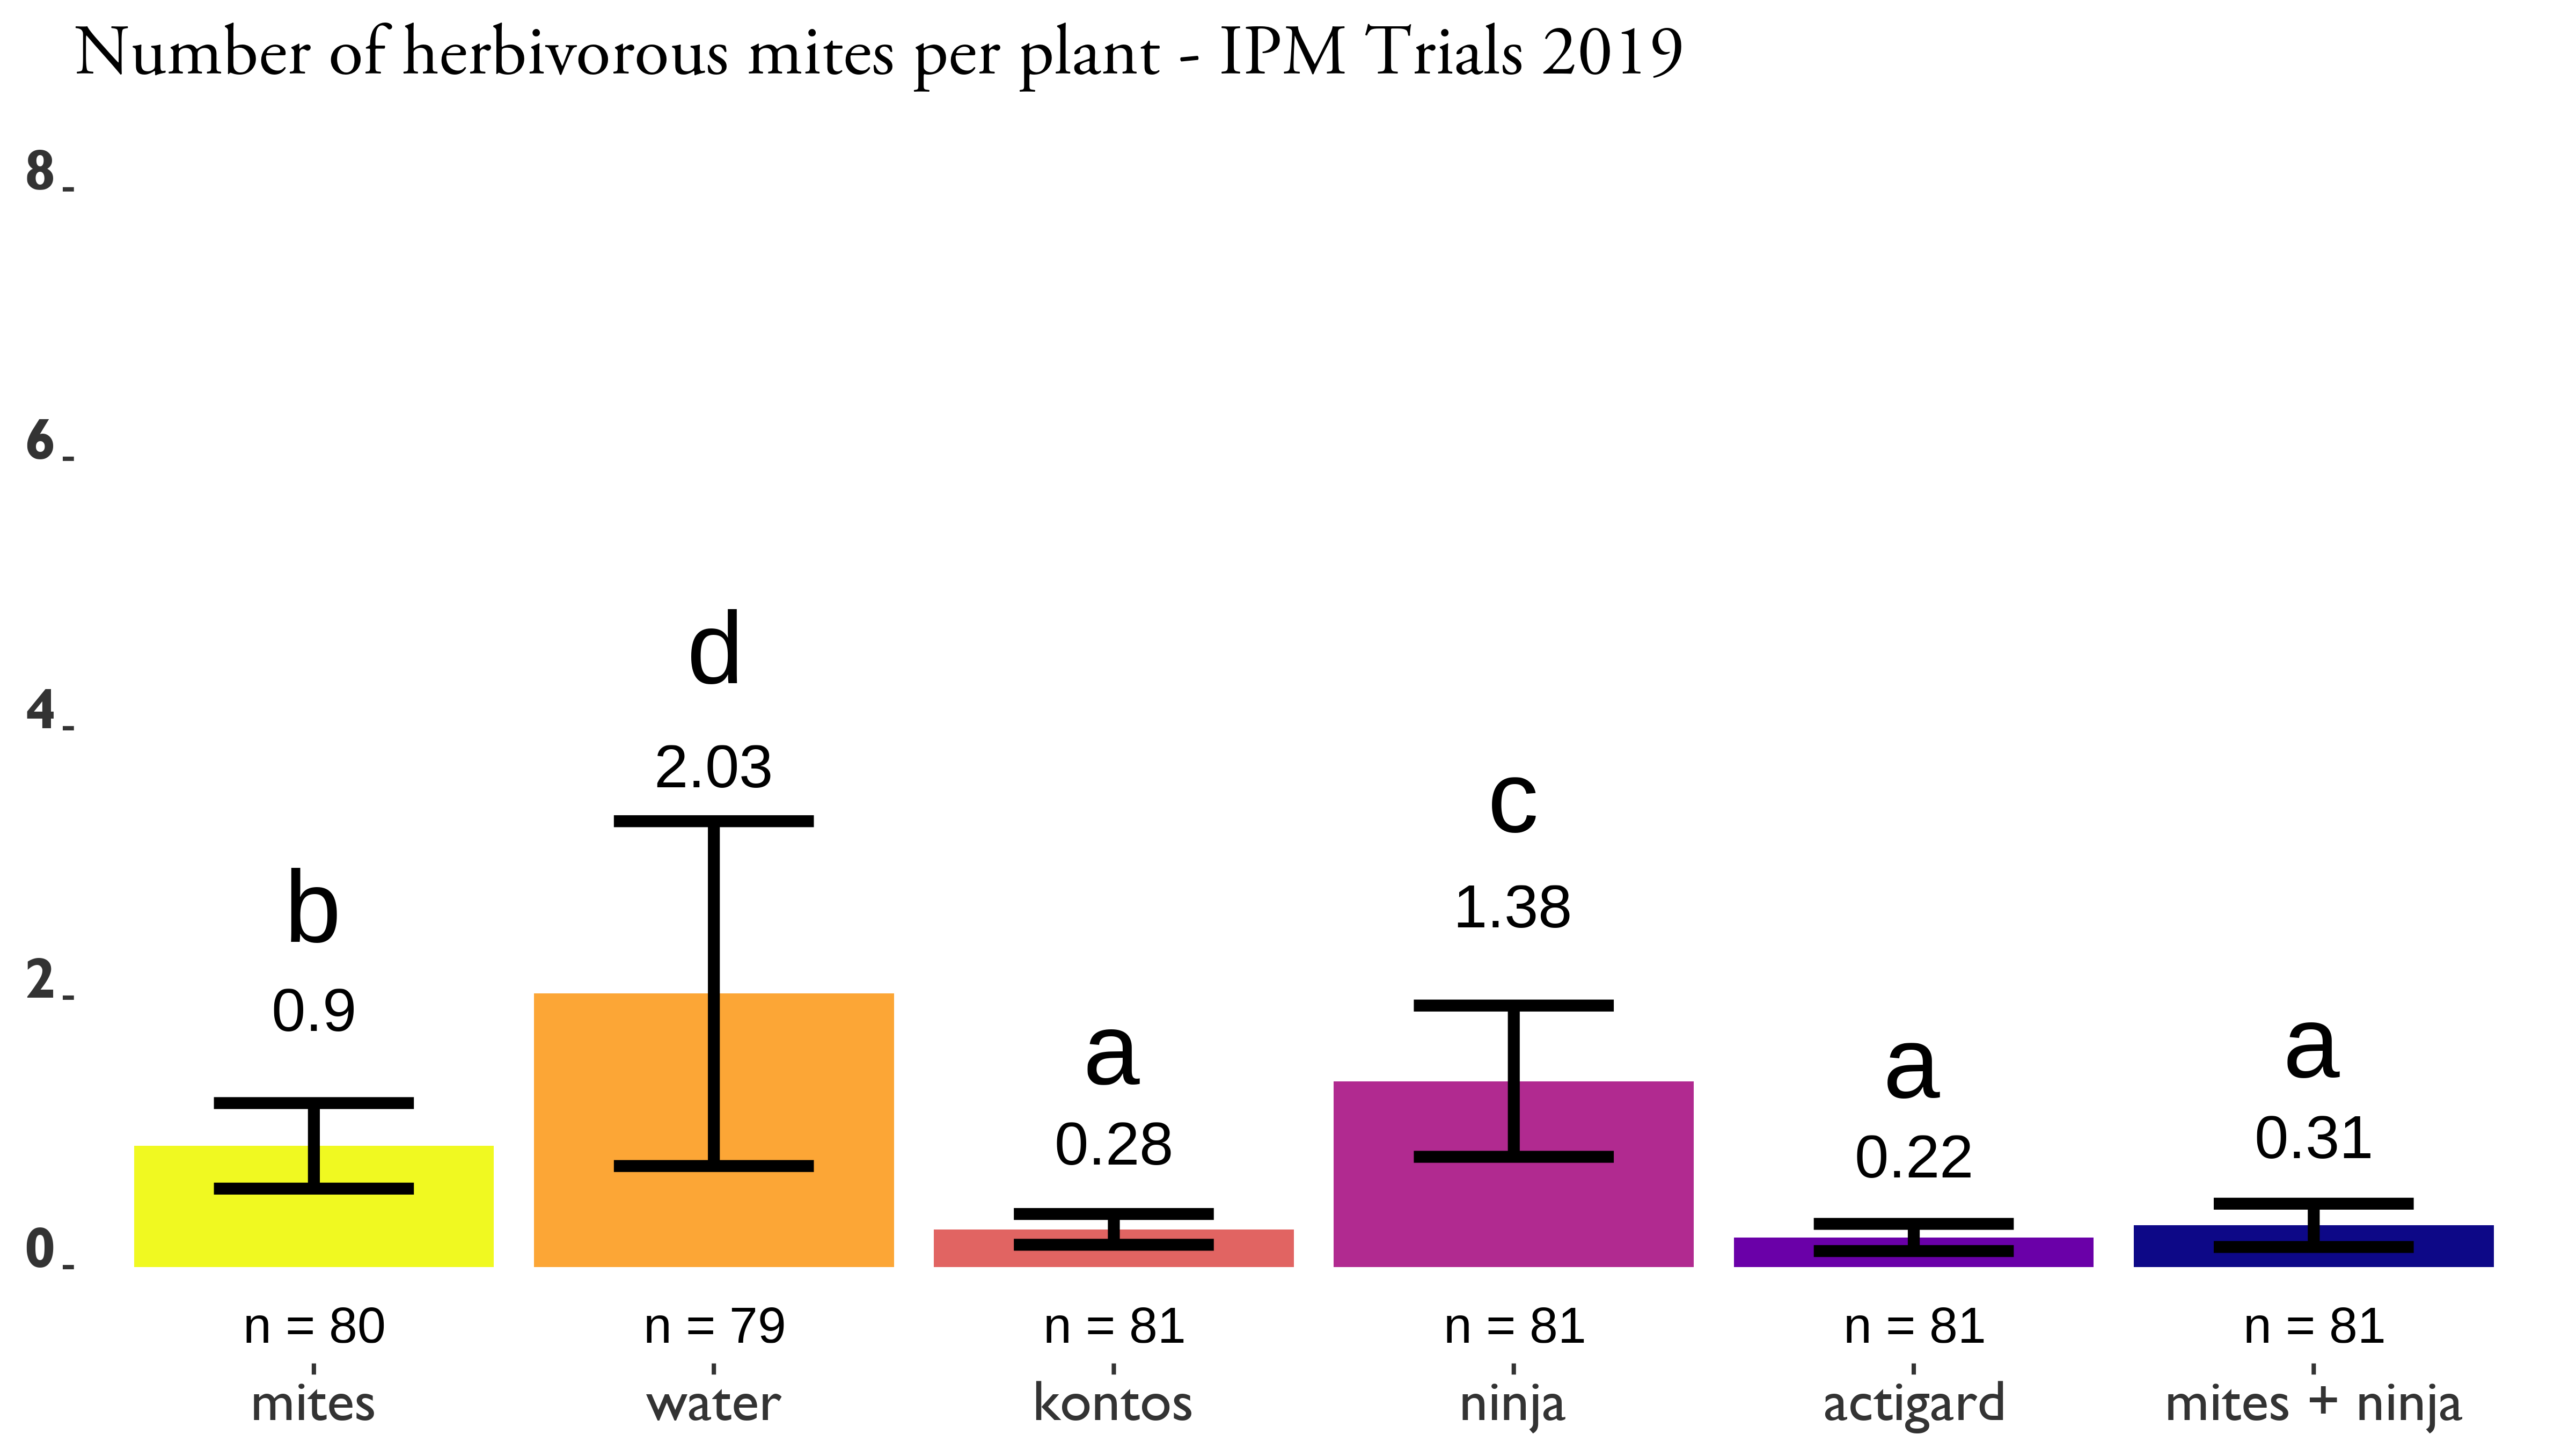
\includegraphics[width=0.8\linewidth]{figure/ipm_graph} \caption{Integrated Pest Management trials on Pink Double Knock Out® roses to control \textit{Phyllocoptes fructiphilus} in Athens and Griffin, GA with five treatments. Statistical significance was determined using Tukey contrasts for multiple Comparisons of means. Groups which share letters are not statistically different from one another. $\alpha = 0.05$. water = Water Control, actigard = Actigard® 50WG (Syngenta, Greensboro, NC, USA) acibenzolar-S-methyl (ASM), kontos = Kontos® Miticide Insecticide - Spirotetramat (Bayer Corporation, Whippany, New Jersey, USA), mites = \textit{Amblyseius swirkii} predatory mite mini sachets on hooks (Ambly-S, Arbico Organics, Oro Valley, AZ, USA), ninja = SP2700 (Trade name: Ninja\texttrademark, SePro, Carmel, IN, USA), mites + ninja = \textit{A. swirskii} + Ninja combined treatments. All products were applied at their label rates for 12 weeks. Flower cuttings were taken weekly to record the numbers of herbivorous mites.}\label{fig:ipm}
\end{figure}
\end{block}

\begin{block}{IPM Trial: Tallahassee 2021}
\protect\hypertarget{ipm-trial-tallahassee-2021}{}
\begin{figure}
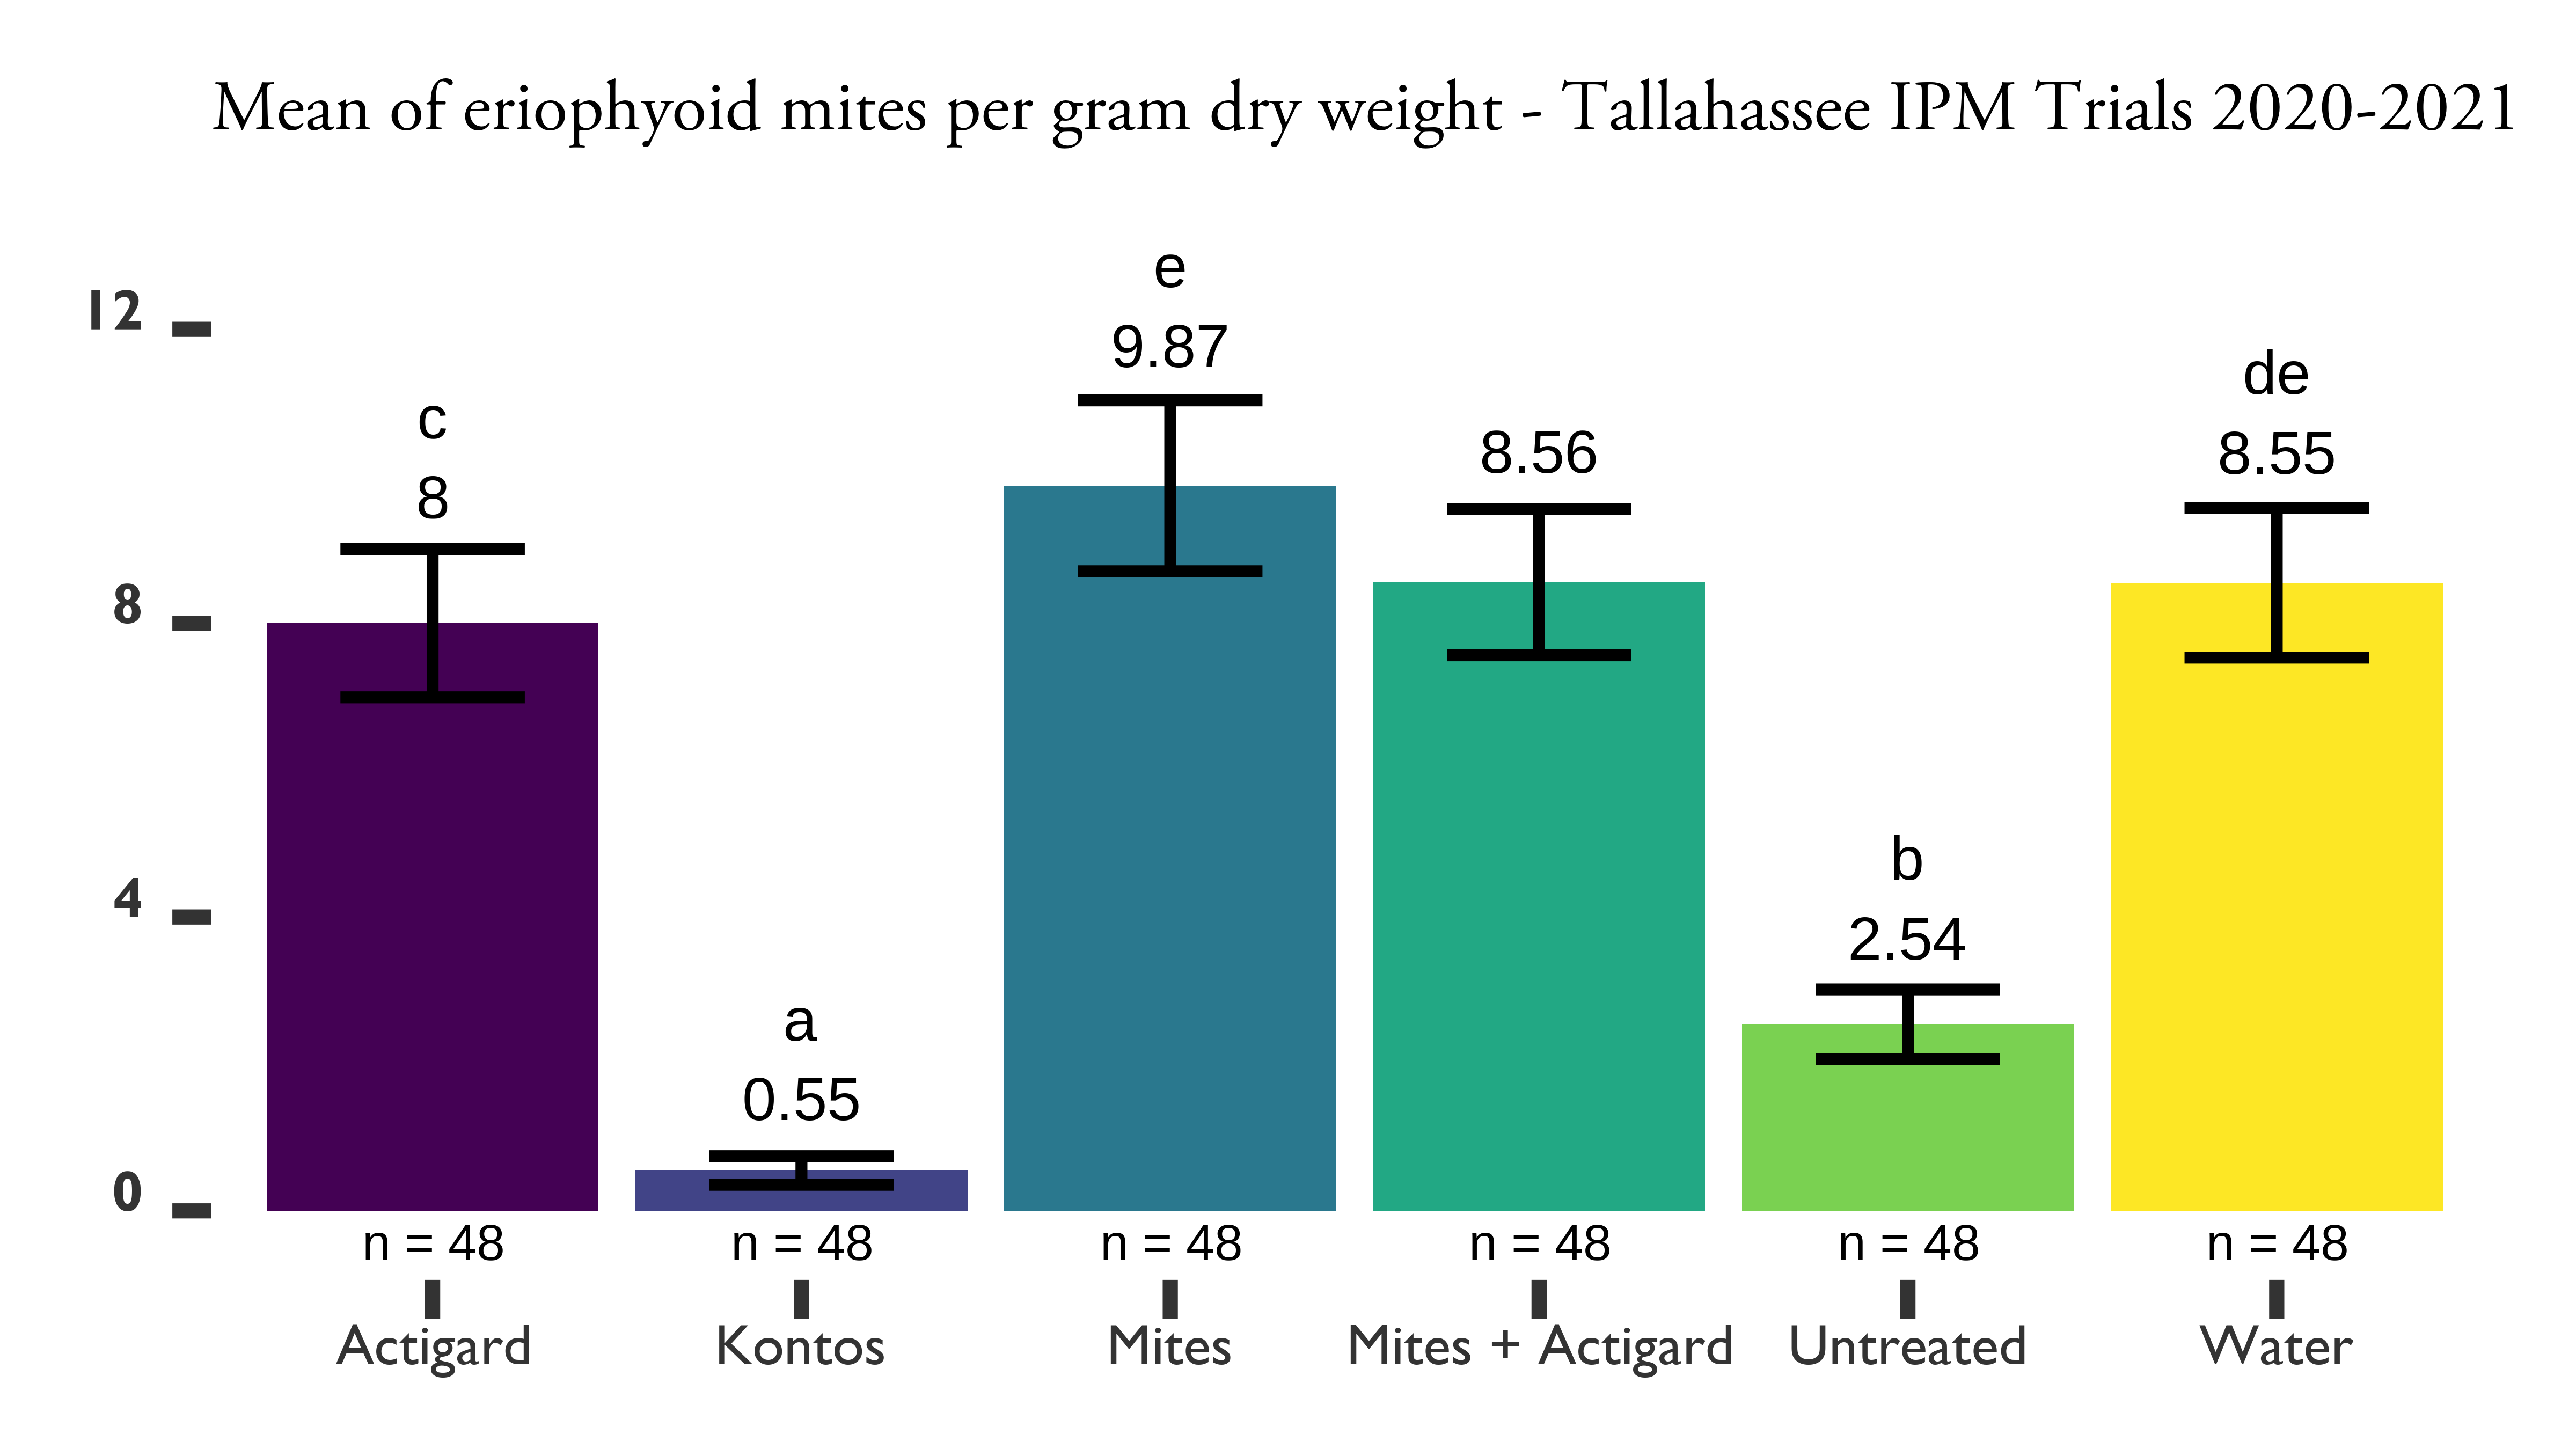
\includegraphics[width=0.8\linewidth]{figure/rrv_ipm_graph_erios_talla} \caption{Integrated Pest Management trials on Pink Double Knock Out® roses to control \textit{Phyllocoptes fructiphilus} in Tallahassee, FL with five treatments. Statistical significance was determined using Tukey contrasts for multiple Comparisons of means. Groups which share letters are not statistically different from one another. $\alpha = 0.05$. Water = Water Control, Actigard = Actigard® 50WG (Syngenta, Greensboro, NC, USA) acibenzolar-S-methyl (ASM), Kontos = Kontos® Miticide Insecticide - Spirotetramat (Bayer Corporation, Whippany, New Jersey, USA), Mites = \textit{Amblyseius swirkii} predatory mite mini sachets on hooks (Ambly-S, Arbico Organics, Oro Valley, AZ, USA), Mites + Actigard = \textit{A. swirskii} + Actigard combined treatments. Untreated = No treatment. All products were applied at their label rates for 12 weeks. Flower cuttings were taken weekly to record the numbers of \textit{P. fructiphilus} and other herbivorous mites.}\label{fig:ipm-talla-erios}
\end{figure}
\end{block}

\begin{block}{IPM Trial: Tallahassee 2021 - week}
\protect\hypertarget{ipm-trial-tallahassee-2021---week}{}
\begin{figure}
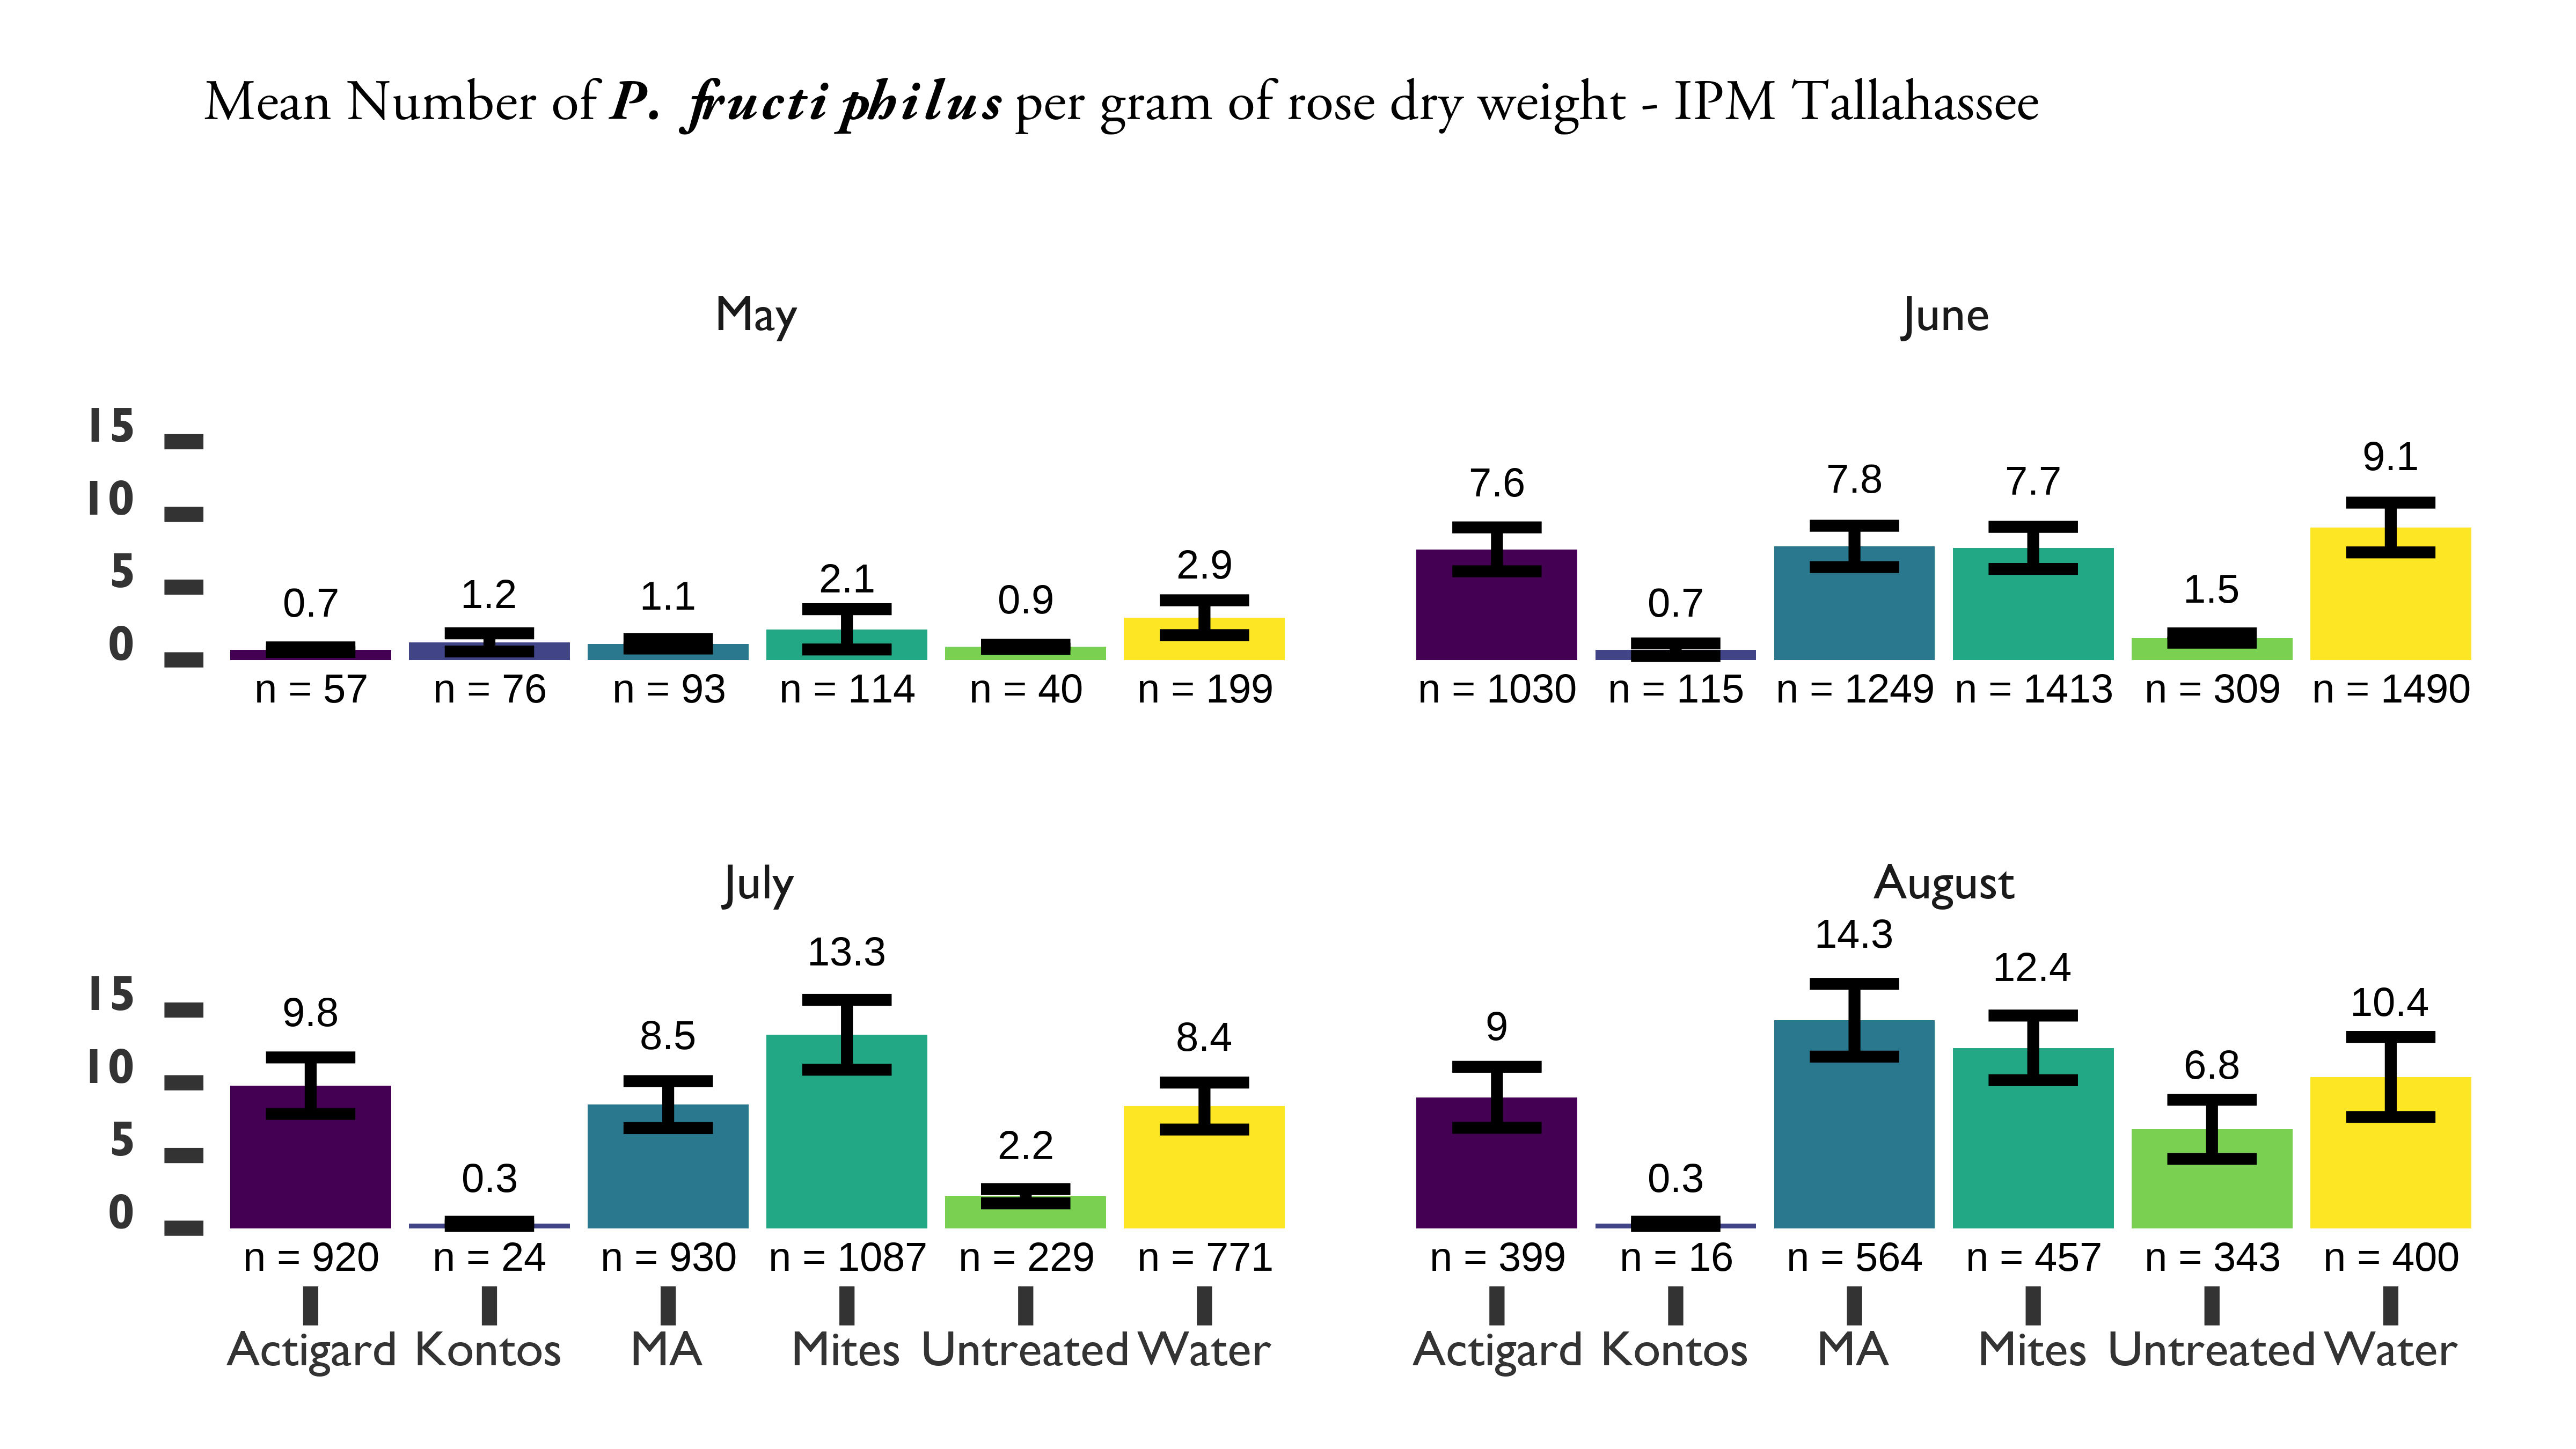
\includegraphics[width=0.8\linewidth]{figure/rrv_ipm_graph_erios_talla_week} \caption{Integrated Pest Management trials on Pink Double Knock Out® roses to control \textit{Phyllocoptes fructiphilus} in Tallahassee, FL with five treatments. Water = Water Control, Actigard = Actigard® 50WG (Syngenta, Greensboro, NC, USA) acibenzolar-S-methyl (ASM), Kontos = Kontos® Miticide Insecticide - Spirotetramat (Bayer Corporation, Whippany, New Jersey, USA), Mites = \textit{Amblyseius swirkii} predatory mite mini sachets on hooks (Ambly-S, Arbico Organics, Oro Valley, AZ, USA), MA = \textit{A. swirskii} + Actigard combined treatments. Untreated = No treatment. All products were applied at their label rates for 12 weeks. Flower cuttings were taken weekly to record the numbers of \textit{P. fructiphilus} and other herbivorous mites.}\label{fig:ipm-talla-erios-week}
\end{figure}
\end{block}

\begin{block}{IPM Trial: Tallahassee 2021 - other}
\protect\hypertarget{ipm-trial-tallahassee-2021---other}{}
\begin{figure}
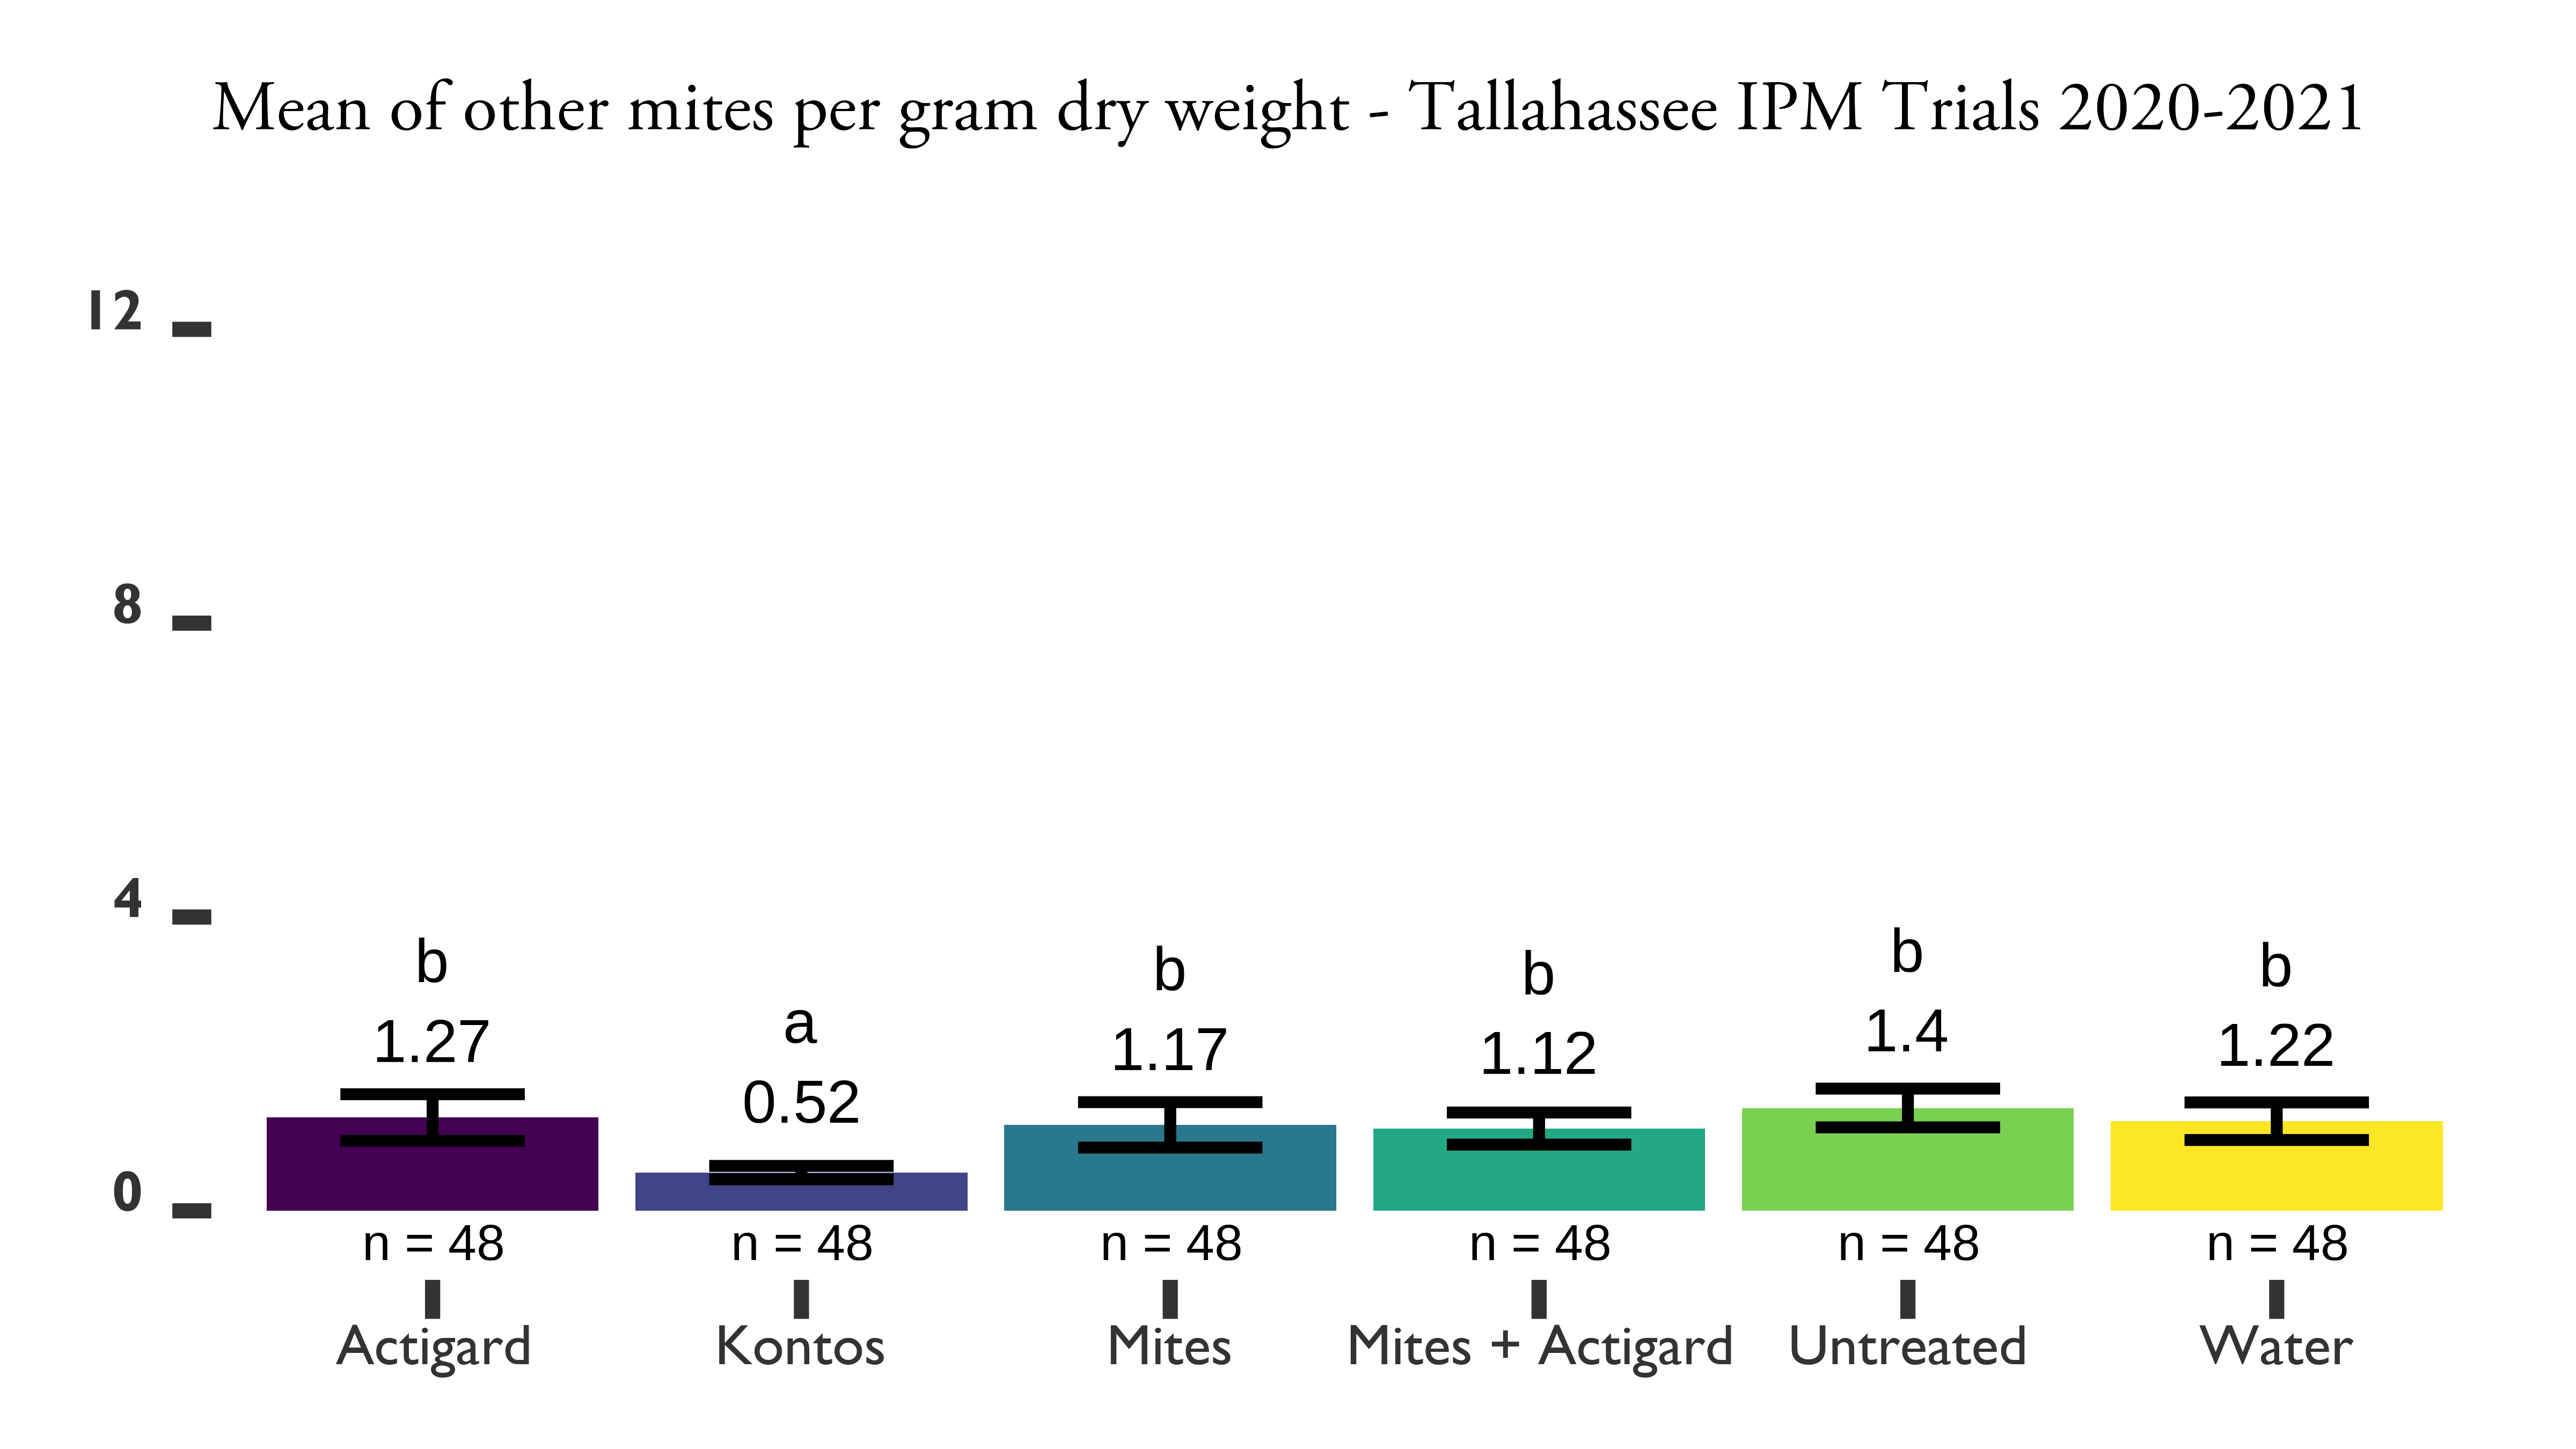
\includegraphics[width=0.8\linewidth]{figure/rrv_ipm_graph_other_talla} \caption{Integrated Pest Management trials on Pink Double Knock Out® roses to control \textit{Phyllocoptes fructiphilus} in Tallahassee, FL with five treatments. Statistical significance was determined using Tukey contrasts for multiple Comparisons of means. Groups which share letters are not statistically different from one another. $\alpha = 0.05$. Water = Water Control, Actigard = Actigard® 50WG (Syngenta, Greensboro, NC, USA) acibenzolar-S-methyl (ASM), Kontos = Kontos® Miticide Insecticide - Spirotetramat (Bayer Corporation, Whippany, New Jersey, USA), Mites = \textit{Amblyseius swirkii} predatory mite mini sachets on hooks (Ambly-S, Arbico Organics, Oro Valley, AZ, USA), Mites + Actigard = \textit{A. swirskii} + Actigard combined treatments. Untreated = No treatment. All products were applied at their label rates for 12 weeks. Flower cuttings were taken weekly to record the numbers of \textit{P. fructiphilus} and other herbivorous mites.}\label{fig:ipm-talla-other}
\end{figure}
\end{block}
\end{frame}

\begin{frame}{Discussion}
\protect\hypertarget{dis-asm-ipm}{}
Our results suggest that SAR-induced plant defenses have the potential
to manage populations of \emph{P. fructiphilus} and other herbivorous
mites, especially when integrating SAR-induction with predatory mites.

\hypertarget{refs}{}
\begin{CSLReferences}{1}{0}
\leavevmode\vadjust pre{\hypertarget{ref-Allington1968}{}}%
\textbf{Allington, W. B., R. Staples, and G. Viehmeyer}. \textbf{1968}.
Transmission of {Rose rosette virus} by the eriophyid mite
{\emph{Phyllocoptes fructiphilus}}. Journal of Economic Entomology. 61:
1137--1140,
DOI:\href{https://doi.org/10.1093/jee/61.5.1137}{10.1093/jee/61.5.1137}.

\leavevmode\vadjust pre{\hypertarget{ref-Amrine1996}{}}%
\textbf{Amrine Jr, J. W.} \textbf{1996}.
\href{https://doi.org/10.1016/s1572-4379(96)80050-9}{{\emph{Phyllocoptes
fructiphilus}} and biological control of multiflora rose}, pp. 741--749.
\emph{In} Helle, W., Lundquist, E.E., Sabelis, M.W., Bruin, J. (eds.),
Eriophyoid Mites. Their Biology, Natural Enemies, and Control, World
Crop Pests. Elsevier.

\leavevmode\vadjust pre{\hypertarget{ref-Amrine2002}{}}%
\textbf{Amrine Jr, J. W.} \textbf{2002}. {\emph{Rosa multiflora}}.
Biological control of invasive plants in the Eastern {United States}.
265--292.

\leavevmode\vadjust pre{\hypertarget{ref-Ataide2016}{}}%
\textbf{Ataide, L. M. S., M. L. Pappas, B. C. J. Schimmel, A.
Lopez-Orenes, J. M. Alba, M. V. A. Duarte, A. Pallini, R. C. Schuurink,
and M. R. Kant}. \textbf{2016}. Induced plant-defenses suppress
herbivore reproduction but also constrain predation of their offspring.
Plant Science. 252: 300--310,
DOI:\href{https://doi.org/10.1016/j.plantsci.2016.08.004}{10.1016/j.plantsci.2016.08.004}.

\leavevmode\vadjust pre{\hypertarget{ref-Bronner1991a}{}}%
\textbf{Bronner, R., E. Westphal, and F. Dreger}. \textbf{1991}.
Pathogenesis-related proteins in {\emph{Solanum dulcamara}} {L.}
Resistant to the gall mite {\emph{Aceria cladophthirus}} ({Nalepa})(syn
{\emph{Eriophyes cladophthirus}} {Nal.}). Physiological and molecular
plant pathology.

\leavevmode\vadjust pre{\hypertarget{ref-Byrne2018}{}}%
\textbf{Byrne, D. H., P. Klein, M. Yan, E. Young, J. Lau, K. Ong, M.
Shires, J. Olson, M. Windham, T. Evans, and D. Novick}. \textbf{2018}.
Challenges of breeding {Rose rosette}-resistant roses. {HortScience}.
53: 604--608,
DOI:\href{https://doi.org/10.21273/hortsci12553-17}{10.21273/hortsci12553-17}.

\leavevmode\vadjust pre{\hypertarget{ref-Bello2017}{}}%
\textbf{Di Bello, P. L., T. Thekke-Veetil, T. Druciarek, and I. E.
Tzanetakis}. \textbf{2017}. Transmission attributes and resistance to
{Rose rosette virus}. Plant Pathology. 67: 499--504,
DOI:\href{https://doi.org/10.1111/ppa.12738}{10.1111/ppa.12738}.

\leavevmode\vadjust pre{\hypertarget{ref-Laney2011}{}}%
\textbf{Laney, A. G., K. E. Keller, R. R. Martin, and I. E. Tzanetakis}.
\textbf{2011}. A discovery 70 years in the making: Characterization of
the {Rose rosette virus}. Journal of General Virology. 92: 1727--1732,
DOI:\href{https://doi.org/10.1099/vir.0.031146-0}{10.1099/vir.0.031146-0}.

\leavevmode\vadjust pre{\hypertarget{ref-Monfreda2007}{}}%
\textbf{Monfreda, R., G. Nuzzaci, and E. De Lillo}. \textbf{2007}.
Detection, extraction, and collection of eriophyoid mites. Zootaxa.
1662: 35--43.

\leavevmode\vadjust pre{\hypertarget{ref-Otero-Colina2018}{}}%
\textbf{Otero-Colina, G., R. Ochoa, J. W. Amrine Jr, J. Hammond, R.
Jordan, and G. R. Bauchan}. \textbf{2018}. Eriophyoid mites found on
healthy and {Rose rosette diseased} roses in the {United States}.
Journal of Environmental Horticulture. 36: 146--153.

\leavevmode\vadjust pre{\hypertarget{ref-Pappas2017}{}}%
\textbf{Pappas, M. L., C. Broekgaarden, G. D. Broufas, M. R. Kant, G. J.
Messelink, A. Steppuhn, F. Wäckers, and N. M. van Dam}. \textbf{2017}.
Induced plant defences in biological control of arthropod pests: A
double-edged sword. Pest Management Science. 73: 1780--1788,
DOI:\href{https://doi.org/10.1002/ps.4587}{10.1002/ps.4587}.

\leavevmode\vadjust pre{\hypertarget{ref-Solo2018}{}}%
\textbf{Solo, K. M.} \textbf{2018}. Rose eriophyid mites: An ecological
study of {\emph{Phyllocoptes fructiphilus}} {Keifer} {({Acari}:
{Eriophyidea})}, vector of {Rose rosette virus}, and its relationship
with {\emph{Rosa}} species (Master's thesis).

\leavevmode\vadjust pre{\hypertarget{ref-Solo2020}{}}%
\textbf{Solo, K. M., S. B. Collins, M. K. Shires, R. Ochoa, G. R.
Bauchan, L. G. Schneider, A. Henn, J. C. Jacobi, J. L.
Williams-Woodward, M. R. Hajimorad, F. A. Hale, J. B. Wilkerson, A. S.
Windham, K. L. Ong, M. L. Paret, X. Martini, D. H. Byrne, and M. T.
Windham}. \textbf{2020}. A survey of {Rose rosette virus} and eriophyid
mites associated with roses in the southeastern {United States}.
{HortScience}. 1--7,
DOI:\href{https://doi.org/10.21273/hortsci14653-20}{10.21273/hortsci14653-20}.

\leavevmode\vadjust pre{\hypertarget{ref-Suo2001}{}}%
\textbf{Suo, Y., and D. W. M. Leung}. \textbf{2001}. Elevation of
extracellular \textbeta-1,3-glucanase and chitinase activities in rose
in response to treatment with acibenzolar-{S}-methyl and infection by
{\emph{D. rosae}}. Journal of Plant Physiology. 158: 971--976,
DOI:\href{https://doi.org/10.1078/0176-1617-00300}{10.1078/0176-1617-00300}.

\leavevmode\vadjust pre{\hypertarget{ref-Tzanetakis2006}{}}%
\textbf{Tzanetakis, I. E., R. C. Gergerich, and R. R. Martin}.
\textbf{2006}. A new {\emph{Ilarvirus}} found in rose. Plant Pathology.
55: 568--568,
DOI:\href{https://doi.org/10.1111/j.1365-3059.2006.01410.x}{10.1111/j.1365-3059.2006.01410.x}.

\leavevmode\vadjust pre{\hypertarget{ref-Westphal1991}{}}%
\textbf{Westphal, E., F. Dreger, and R. Bronner}. \textbf{1991}. Induced
resistance in {\emph{Solanum dulcamara}} triggered by the gall mite
{\emph{Aceria cladophthirus}} ({Acari}: {Eriophyoidea}). Experimental
{\&} Applied Acarology. 12: 111--118,
DOI:\href{https://doi.org/10.1007/bf01204404}{10.1007/bf01204404}.

\leavevmode\vadjust pre{\hypertarget{ref-Westphal1992}{}}%
\textbf{Westphal, E., M. J. Perrot-Minnot, S. Kreiter, and J.
Gutierrez}. \textbf{1992}. Hypersensitive reaction of {\emph{Solanum
dulcamara}} to the gall mite {\emph{Aceria cladophthirus}} causes an
increased susceptibility to {\emph{Tetranychus urticae}}. Experimental
{\&} Applied Acarology. 15: 15--26,
DOI:\href{https://doi.org/10.1007/bf01193964}{10.1007/bf01193964}.

\end{CSLReferences}
\end{frame}

\end{document}
